%%%%%%%%%%%%%%%%%%%%%%%%%%%%%%%%%%%%%%%%%
% Masters/Doctoral Thesis
% LaTeX Template
% Version 2.5 (27/8/17)
%
% This template was downloaded from:
% http://www.LaTeXTemplates.com
%
% Version 2.x major modifications by:
% Vel (vel@latextemplates.com)
%
% This template is based on a template by:
% Steve Gunn (http://users.ecs.soton.ac.uk/srg/softwaretools/document/templates/)
% Sunil Patel (http://www.sunilpatel.co.uk/thesis-template/)
%
% Template license:
% CC BY-NC-SA 3.0 (http://creativecommons.org/licenses/by-nc-sa/3.0/)
%
%%%%%%%%%%%%%%%%%%%%%%%%%%%%%%%%%%%%%%%%%

%----------------------------------------------------------------------------------------
%	PACKAGES AND OTHER DOCUMENT CONFIGURATIONS
%----------------------------------------------------------------------------------------

\documentclass[
11pt, % The default document font size, options: 10pt, 11pt, 12pt
%oneside, % Two side (alternating margins) for binding by default, uncomment to switch to one side
english, % ngerman for German
singlespacing, % Single line spacing, alternatives: onehalfspacing or doublespacing
%draft, % Uncomment to enable draft mode (no pictures, no links, overfull hboxes indicated)
%nolistspacing, % If the document is onehalfspacing or doublespacing, uncomment this to set spacing in lists to single
%liststotoc, % Uncomment to add the list of figures/tables/etc to the table of contents
%toctotoc, % Uncomment to add the main table of contents to the table of contents
%parskip, % Uncomment to add space between paragraphs
%nohyperref, % Uncomment to not load the hyperref package
headsepline, % Uncomment to get a line under the header
%chapterinoneline, % Uncomment to place the chapter title next to the number on one line
%consistentlayout, % Uncomment to change the layout of the declaration, abstract and acknowledgements pages to match the default layout
openany,
]{MastersDoctoralThesis} % The class file specifying the document structure

\usepackage[utf8]{inputenc} % Required for inputting international characters
\usepackage[T1]{fontenc} % Output font encoding for international characters
\usepackage{textcomp}
\usepackage{amsmath,amssymb}
\usepackage{mathpazo} % Use the Palatino font by default
\usepackage[version=4]{mhchem}
%\usepackage[backend=bibtex,style=authoryear,natbib=true]{biblatex} % Use the bibtex backend with the authoryear citation style (which resembles APA)
% The filename of the bibliography
\usepackage{booktabs}
\usepackage{caption}
\usepackage{subcaption}
\usepackage{enumitem}
\usepackage{float}
\usepackage[autostyle=true]{csquotes} % Required to generate language-dependent quotes in the bibliography
\usepackage{tikz}
\usetikzlibrary{shapes,arrows}
\usetikzlibrary{arrows,arrows.meta,calc,positioning}

\tikzset{
    block/.style = {draw, rectangle,
        minimum height=1cm,
        minimum width=2cm},
    input/.style = {coordinate,node distance=1cm},
    output/.style = {coordinate,node distance=4cm},
    arrow/.style={draw, -latex,node distance=2cm},
    pinstyle/.style = {pin edge={latex-, black,node distance=2cm}},
    sum/.style = {draw, circle, node distance=1cm}
}
\makeatletter
\def\endthebibliography{%
	\def\@noitemerr{\@latex@warning{Empty `thebibliography' environment}}%
	\endlist
}
%----------------------------------------------------------------------------------------
%	MARGIN SETTINGS
%----------------------------------------------------------------------------------------

\usepackage{graphicx}

\geometry{
	paper=a4paper, % Change to letterpaper for US letter
	inner=1.5cm, % Inner margin (report rules: 1.5 cm on all sides)
	outer=1.5cm, % Outer margin
	bindingoffset=0cm, % Binding offset
	top=1cm, % Top margin
	bottom=1cm, % Bottom margin
	%showframe, % Uncomment to show how the type block is set on the page
}

%----------------------------------------------------------------------------------------
%	THESIS INFORMATION
%----------------------------------------------------------------------------------------

\thesistitle{Modeling and Control of a PEM Fuel Cell Stack} % Your thesis title, this is used in the title and abstract, print it elsewhere with \ttitle
\supervisor{Prof. Emmanuel \textsc{WITRANT}} % Your supervisor's name, this is used in the title page, print it elsewhere with \supname
\examiner{} % Your examiner's name, this is not currently used anywhere in the template, print it elsewhere with \examname
\degree{} % Your degree name, this is used in the title page and abstract, print it elsewhere with \degreename
\author{Khalil Ellah \textsc{LAGHA}} % Your name, this is used in the title page and abstract, print it elsewhere with \authorname
\addresses{} % Your address, this is not currently used anywhere in the template, print it elsewhere with \addressname

\subject{} % Your subject area, this is not currently used anywhere in the template, print it elsewhere with \subjectname
\keywords{} % Keywords for your thesis, this is not currently used anywhere in the template, print it elsewhere with \keywordnames
\university{\href{http://www.university.com}{ Universit\'e Grenoble Alpes}} % Your university's name and URL, this is used in the title page and abstract, print it elsewhere with \univname
\department{\href{http://department.university.com}{}} % Your department's name and URL, this is used in the title page and abstract, print it elsewhere with \deptname
\group{\href{http://researchgroup.university.com}{Infinity Team - Gipsa}} % Your research group's name and URL, this is used in the title page, print it elsewhere with \groupname
\faculty{\href{http://faculty.university.com}{}} % Your faculty's name and URL, this is used in the title page and abstract, print it elsewhere with \facname

\AtBeginDocument{
\hypersetup{pdftitle=\ttitle} % Set the PDF's title to your title
\hypersetup{pdfauthor=\authorname} % Set the PDF's author to your name
\hypersetup{pdfkeywords=\keywordnames} % Set the PDF's keywords to your keywords
}
\usepackage{multicol}
\begin{document}

\frontmatter % Use roman page numbering style (i, ii, iii, iv...) for the pre-content pages

\pagestyle{plain} % Default to the plain heading style until the thesis style is called for the body content

%----------------------------------------------------------------------------------------
%	TITLE PAGE
%----------------------------------------------------------------------------------------

\begin{titlepage}
\begin{center}

\vspace*{.04\textheight}
\begin{minipage}{0.45\textwidth}
\begin{flushleft}

\includegraphics[height=2cm]{Figures/UGAlogo.png}
\end{flushleft}
\end{minipage}
\hfill
\begin{minipage}{0.45\textwidth}
\begin{flushright}

\includegraphics[height=2cm]{Figures/gipsa-lablogo.jpg}
\end{flushright}
\end{minipage}\\[1.2cm]

{\scshape\LARGE \univname\par}\vspace{1.5cm} % University name
\textsc{\Large Internship Report}\\[0.5cm] % Thesis type

\HRule \\[0.4cm] % Horizontal line
{\huge \bfseries \ttitle\par}\vspace{0.4cm} % Thesis title
\HRule \\[1.5cm] % Horizontal line

\begin{minipage}[t]{0.4\textwidth}
\begin{flushleft} \large
\emph{Author:}\\
\authorname
\end{flushleft}
\end{minipage}
\begin{minipage}[t]{0.4\textwidth}
\begin{flushright} \large
\emph{Supervisor:} \\
\supname
\end{flushright}
\end{minipage}\\[3cm]

\vfill

\large \textit{\degreename}\\[0.3cm] % University requirement text
\textit{}\\[0.4cm]
\groupname\\[2cm] % Research group name and department name

\vfill

{\large \today}\\[4cm] % Date
%\includegraphics{Logo} % University/department logo - uncomment to place it

\vfill
\end{center}
\end{titlepage}

%----------------------------------------------------------------------------------------
%	DECLARATION PAGE
%----------------------------------------------------------------------------------------

\begin{declaration}
\addchaptertocentry{\authorshipname} % Add the declaration to the table of contents
\noindent I, \authorname, declare that this thesis titled, \enquote{\ttitle} and the work presented in it are my own. I confirm that:

\begin{itemize}
\item This work was done wholly or mainly while in candidature for a research degree at this University.
\item Where any part of this thesis has previously been submitted for a degree or any other qualification at this University or any other institution, this has been clearly stated.
\item Where I have consulted the published work of others, this is always clearly attributed.
\item Where I have quoted from the work of others, the source is always given. With the exception of such quotations, this thesis is entirely my own work.
\item I have acknowledged all main sources of help.
\item Where the thesis is based on work done by myself jointly with others, I have made clear exactly what was done by others and what I have contributed myself.\\
\end{itemize}

\noindent Signed:\\
\rule[0.5em]{25em}{0.5pt} % This prints a line for the signature

\noindent Date:\\
\rule[0.5em]{25em}{0.5pt} % This prints a line to write the date
\end{declaration}

\cleardoublepage

%----------------------------------------------------------------------------------------
%	QUOTATION PAGE
%----------------------------------------------------------------------------------------

\vspace*{0.2\textheight}

\noindent\enquote{\itshape Where there is a will there's a way.}\bigbreak

\hfill George Herbert

%----------------------------------------------------------------------------------------
%	ABSTRACT PAGE
%----------------------------------------------------------------------------------------

\begin{abstract}
\addchaptertocentry{\abstractname}
This report presents the modeling, calibration, and dynamic characterization of a
proton exchange membrane fuel cell (PEMFC) stack carried out at GIPSA-lab.
A simplified control-oriented model is developed from electrochemical principles:
a Nernst open-circuit voltage combined with semi-empirical activation, ohmic, and
concentration losses, coupled to lumped-volume hydrogen, membrane-hydration, and
cathode-humidity dynamics. Six parameters per cell are identified from the
Optimization Experiment using a two-stage optimization (differential evolution
followed by L-BFGS-B), yielding root-mean-square voltage errors below 12\,mV for
all healthy cells and revealing degraded cells through voltage collapse and
degenerate fits. The state-space matrices of the linearized model are written out
explicitly --- the state and input matrices follow directly from the dynamic
equations, while the output matrices require a Jacobian linearization of the
nonlinear voltage equation. The system is shown to be structurally controllable
for all realistic electro-osmotic drag coefficients, while a voltage-only output
observes the hydrogen pressure but not the water states. Step-load experiments
(3.3\,$\Omega$ and 6.8\,$\Omega$) characterize the current response of the stack
($\tau_I \approx 8$--$10$\,s), providing quantitative targets for closed-loop
control design. Building on these results, a control architecture based on a
DC/DC boost converter regulated by a PI controller is presented, in which the
converter output is regulated to behave either as a current source --- the
approach of Derbeli et al.\ --- or as a voltage source. Results are presented in
the body; the open-circuit-voltage derivation and the full per-cell parameter
table are gathered in the appendices.
\end{abstract}

%----------------------------------------------------------------------------------------
%	ACKNOWLEDGEMENTS
%----------------------------------------------------------------------------------------

\begin{acknowledgements}
\addchaptertocentry{\acknowledgementname}
I would like to thank my supervisor, Prof.~Emmanuel Witrant, and the Infinity Team
at GIPSA-lab for their guidance and support throughout this internship.
\end{acknowledgements}

%----------------------------------------------------------------------------------------
%	LIST OF CONTENTS/FIGURES/TABLES PAGES
%----------------------------------------------------------------------------------------

\tableofcontents % Prints the main table of contents

\listoffigures % Prints the list of figures

\listoftables % Prints the list of tables

%----------------------------------------------------------------------------------------
%	THESIS CONTENT - CHAPTERS
%----------------------------------------------------------------------------------------

\mainmatter % Begin numeric (1,2,3...) page numbering

\pagestyle{thesis} % Return the page headers back to the "thesis" style

% Include the chapters of the thesis as separate files from the Chapters folder

% Chapter 1 — Introduction

\chapter{Introduction}

\label{Chapter1}

Fuel cells convert the chemical energy of hydrogen directly into electricity, with
water and heat as the only by-products. Among them, the proton exchange membrane
fuel cell (PEMFC) is the leading candidate for transport and small stationary
applications thanks to its low operating temperature, high power density, and fast
start-up \cite{pukrushpan2003,daud2017pem}. Their efficient and safe operation,
however, requires feedback control of the gas supply and load: insufficient
reactant flow causes starvation and irreversible degradation, while excessive
anode--cathode pressure difference can damage the membrane \cite{zhu2017,kharrat2025}.
Control design, in turn, requires a model that is simple enough for analysis and
accurate enough to represent the actual hardware --- including the differences
between individual cells of a stack \cite{manana2006}.

This internship, carried out at GIPSA-lab (Universit\'e Grenoble Alpes) under the
supervision of Prof.~Emmanuel Witrant, addresses this need for a small educational
PEMFC stack of ten cells. The objectives are:
\begin{enumerate}[label=\arabic*)]
    \item to develop a simplified, control-oriented dynamic model of a single cell
          and of the stack, grounded in the electrochemical literature;
    \item to identify the model parameters \emph{per cell} from experimental data
          acquired on the bench;
    \item to derive the linearized state-space representation and analyze its
          structural controllability and observability, as a foundation for
          controller and observer design;
    \item to characterize experimentally the dynamic response of the stack to
          resistive load steps, providing the timescales needed for control
          bandwidth selection;
    \item to propose a PI-based control architecture for the PEMFC power system
          through a DC/DC boost converter, following \cite{derbeli2017}.
\end{enumerate}

The report is organized to give a global vision of the work.
Chapter~\ref{Chapter2} summarizes the operating principle of PEMFCs, positions the
work in the literature, and explains the practical constraints that shaped the
control strategy. Chapter~\ref{Chapter3} presents the simplified model, the
parameter-identification procedure, the linearized state-space analysis, and the
experimental protocols. Chapter~\ref{Chapter4} discusses the calibration and
step-response results. Chapter~\ref{Chapter5} presents the control of the PEMFC
power system with a DC/DC boost converter and a PI controller.
Chapter~\ref{Chapter6} concludes and outlines perspectives. The
open-circuit-voltage derivation and the full per-cell parameter table are provided
in Appendices~\ref{app:ocv} and~\ref{app:tables}; the main text is self-contained
and readable without them.

% Chapter 2 — Context & Background

\chapter{Context \& Background}

\label{Chapter2}

\section{Operating Principle of a PEM Fuel Cell}

A proton exchange membrane fuel cell (PEMFC) converts the chemical energy of
hydrogen and oxygen directly into electricity, heat, and water
\cite{manana2006,mohiuddin2018,thomya2011}. At the anode, hydrogen splits into
protons and electrons. The protons cross the polymer membrane, while the
electrons travel through the external circuit and supply the load. At the
cathode, oxygen recombines with both to form water (Figure~\ref{fig:pemfc-operation}).
The overall reaction is
\begin{equation*}
    \mathrm{H_2 + \tfrac{1}{2}O_2 \rightarrow H_2O + electricity + heat}.
\end{equation*}
The membrane conducts protons, blocks electrons, and separates fuel from
oxidant. Together with the two electrodes it forms the membrane electrode
assembly (MEA), the elementary repeating unit of the stack
\cite{manana2006,ionescu2020}. Water management is critical to performance: a dry
membrane loses proton conductivity, whereas excess liquid water floods the gas
channels. Stable operation therefore requires a balance between hydration and
drainage \cite{weber2004,zhang2017}.

\begin{figure}[t]
    \centering
    \begin{subfigure}[t]{0.56\linewidth}
        \centering
        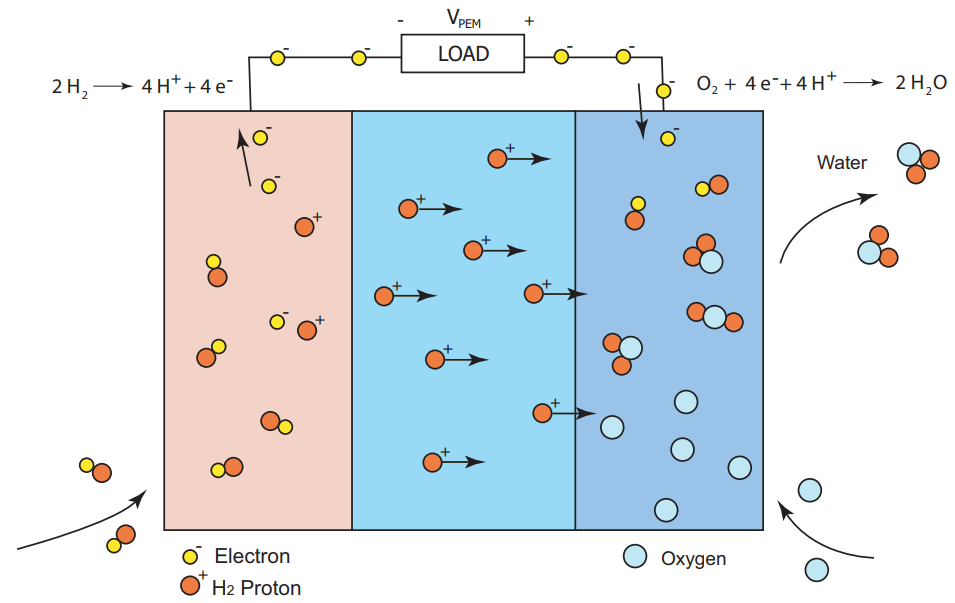
\includegraphics[width=\linewidth]{Figures/pemfc_operation.png}
        \caption{Electrochemical operation: hydrogen oxidation at the anode,
                 proton transport through the membrane, oxygen reduction at the
                 cathode.}
    \end{subfigure}
    \hfill
    \begin{subfigure}[t]{0.38\linewidth}
        \centering
        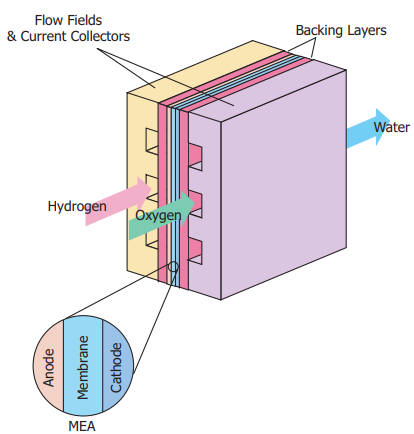
\includegraphics[width=\linewidth]{Figures/pemfc_stack_structure.png}
        \caption{Stack structure: individual MEAs stacked in series to add their
                 voltages.}
    \end{subfigure}
    \caption[Operating principle and structure of a PEM fuel cell]{Operating
             principle and physical structure of a PEM fuel cell. A single cell
             delivers roughly one volt, so cells are stacked in series to reach a
             useful voltage \cite{mohiuddin2018,thomya2011,manana2006}.}
    \label{fig:pemfc-operation}
\end{figure}

\section{Voltage Losses and Polarization Behavior}

A practical cell delivers less than its reversible (open-circuit) voltage because
of three loss mechanisms, each dominant in a different region of the polarization
curve (Figure~\ref{fig:pemfc-losses}) \cite{manana2006,pukrushpan2003,thanapalan2008}:
\begin{itemize}
    \item \textbf{activation loss} --- the kinetic penalty of driving the
          electrode reactions, dominant at low current \cite{pukrushpan2003,weber2004};
    \item \textbf{ohmic loss} --- the resistive drop across the membrane and
          conductors, approximately linear in current \cite{pukrushpan2003,thanapalan2008};
    \item \textbf{concentration loss} --- the mass-transport limitation that
          causes the steep voltage drop at high current \cite{manana2006,weber2004}.
\end{itemize}
The \emph{polarization curve} is the cell voltage plotted against current density;
it is the fingerprint of cell performance and the basis for the model of
Chapter~\ref{Chapter3}. Fast transients are further shaped by the charge
double-layer at the electrode/electrolyte interface, which behaves as a small
capacitor in equivalent-circuit models \cite{pukrushpan2003,manana2006}.

\begin{figure}[t]
    \centering
    \begin{subfigure}[t]{0.48\linewidth}
        \centering
        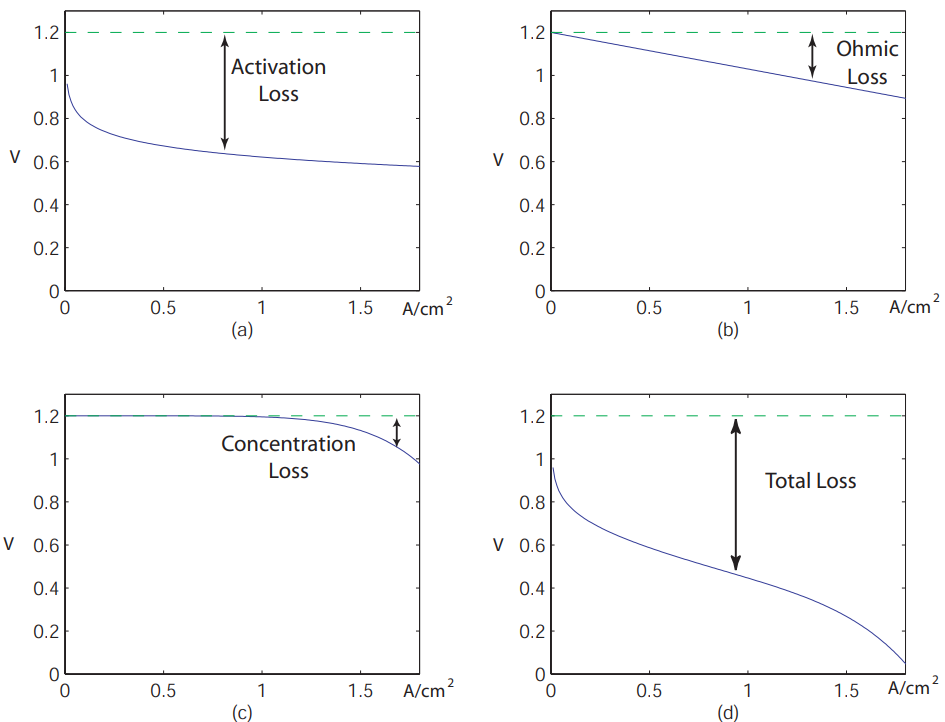
\includegraphics[width=\linewidth]{Figures/pemfc_loss_components.png}
        \caption{Decomposition into activation, ohmic, and concentration losses.}
    \end{subfigure}
    \hfill
    \begin{subfigure}[t]{0.48\linewidth}
        \centering
        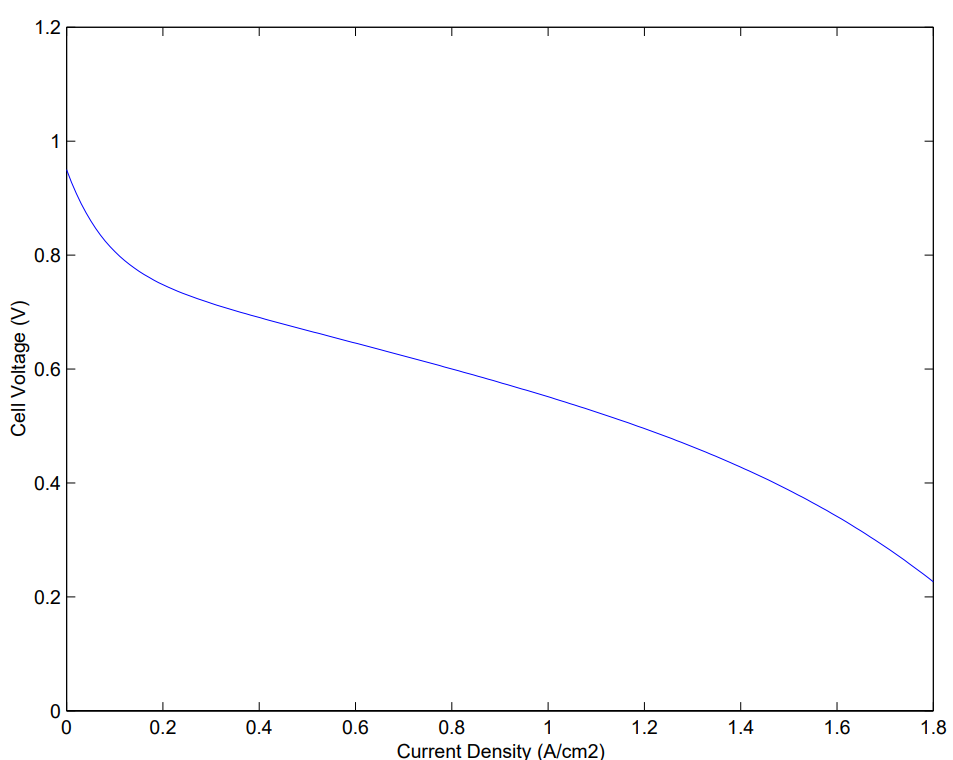
\includegraphics[width=\linewidth]{Figures/pemfc_polarization_curve.png}
        \caption{Resulting polarization curve.}
    \end{subfigure}
    \caption[Voltage losses and polarization curve]{Influence of the three loss
             mechanisms on PEMFC performance. Activation dominates at low current,
             ohmic loss in the middle, and concentration loss near the limiting
             current --- together they bend the ideal flat voltage into the
             characteristic polarization curve.}
    \label{fig:pemfc-losses}
\end{figure}

\section{State of the Art}
\label{sec:sota}

Control-oriented PEMFC modeling traces back to the system-level model of
Pukrushpan \cite{pukrushpan2003}, which couples a polarization-curve voltage law
with compressor, manifold-filling, and membrane-hydration dynamics; most later
models specialize or simplify it \cite{thanapalan2008,kim2010,zhu2017}. Simplified
electrical models reproduce the static voltage--current characteristic of small
stacks with only a handful of parameters \cite{manana2006,shen2005}. Crucially,
per-cell measurements on a small stack reveal voltage deviations of up to 7\,\%
between cells \cite{manana2006}, which motivates the per-cell calibration adopted
here. Parameter identification by direct-search optimization on measured voltage
and power was formalized by Thanapalan et al.\ \cite{thanapalan2008} and extended
with modern metaheuristics \cite{cao2019}.

On the control side, proportional--integral (PI) regulation of flows, pressures,
and converter currents is the established baseline \cite{zhu2017,derbeli2017}.
Documented upgrades include linear-quadratic (LQ) multivariable control,
time-delay control, and model-predictive schemes
\cite{pukrushpan2003,kim2010,wang2021simulation}. At system level, the response
delays of the air and hydrogen supply components remain the main factor limiting
dynamic operation \cite{kharrat2025}.

\subsection{Practical Challenges and Choice of Control Strategy}
\label{sec:challenges}

The control strategy of this work was shaped directly by constraints observed on
the laboratory bench. The most natural actuator for a fuel cell is the hydrogen
supply: raising the anode pressure raises the Nernst voltage and the available
current. In practice, however, the usable hydrogen pressure on the educational
stack is narrowly bounded. The supply regulator caps the inlet pressure, and a
large anode--cathode pressure difference risks mechanical damage to the thin
membrane \cite{zhu2017,kharrat2025}. The pressure can therefore be varied only
within a small range, which yields too little authority to regulate the operating
point across the full load. Direct current control through the hydrogen valve was
explored and found impractical for the same reason: the actuator saturates before
the load demand is met.

This limitation motivated the chosen approach. Rather than acting on the slow,
saturation-limited gas supply, the control is moved to the electrical side: the
stack feeds a DC/DC boost converter whose duty cycle is set by a fast PI loop
\cite{derbeli2017}. The converter decouples the load from the cell and shapes the
delivered power, while the hydrogen supply is left to maintain an adequate
pressure rather than to track the load. This separation of roles --- electrical
control for the fast dynamics, gas supply for the slow operating conditions ---
underlies the architecture developed in Chapter~\ref{Chapter5}.

% Chapter 3 — Methodology

\chapter{Methodology}

\label{Chapter3}

\section{Simplified Control-Oriented Model}
\label{sec:model}

Following \cite{thanapalan2008,pukrushpan2003}, the cell is split into three
interacting parts --- anode, membrane, and cathode --- each lumped into a single
control volume. The main assumptions are: hydrogen and air are the only
reactants; channel pressure drops are neglected; gases obey the ideal-gas law;
temperature is constant or slowly varying; and the oxygen partial pressure is
fixed at $P_{O_2}^{\ast}=0.21\,P_{\mathrm{atm}}$. The result is a simplified
semi-empirical model: physically motivated mass balances combined with empirical
loss laws calibrated from data \cite{cao2019}.

\subsection{Open-Circuit Voltage}
The reversible (open-circuit) voltage follows from the Gibbs free energy of the
reaction and Faraday's law (full derivation in Appendix~\ref{app:ocv}):
\begin{equation}
    \label{eq:ocv}
    E = 1.229 - 0.85\times10^{-3}(T_{fc}-298.15)
      + 4.31\times10^{-5}\,T_{fc}\left[\ln p_{H_2} + \tfrac{1}{2}\ln p_{O_2}\right]\;\mathrm{V},
\end{equation}
with $T_{fc}$ the stack temperature [K] and $p_{H_2}$, $p_{O_2}$ the reactant
partial pressures [atm] \cite{pukrushpan2003}.

\subsection{Voltage Losses}
The cell voltage is the reversible voltage minus the three losses of
Section~\ref{sec:sota}:
\begin{equation}
    \label{eq:vfc}
    v_{fc} = E - v_{act} - v_{ohm} - v_{con},
\end{equation}
with the semi-empirical forms \cite{pukrushpan2003,thanapalan2008,cao2019}
\begin{align}
    v_{act} &= \xi_1+\xi_2 T+\xi_3 T\ln(C_{O_2})+\xi_4 T\ln(i_{FC}),
    \label{eq:vact}\\
    v_{ohm} &= i_{FC}\Bigl(\rho_m\frac{t_m}{A_{fc}}+c\Bigr),
    \qquad
    \rho_m = \Bigl[(b_{11}\lambda_m-b_{12})
              \exp\bigl(b_2(\tfrac{1}{303}-\tfrac{1}{T_{fc}})\bigr)\Bigr]^{-1},
    \label{eq:vohm}\\
    v_{con} &= -B\ln\Bigl(1-\frac{i_{FC}}{i_{\max}}\Bigr),
    \label{eq:vcon}
\end{align}
where $i_{FC}$ is the cell current, $C_{O_2}$ the dissolved-oxygen concentration
(Henry's law), $t_m$ and $A_{fc}$ the membrane thickness and active area,
$\lambda_m$ the membrane water content, and
$\boldsymbol{\theta}=(\xi_1,\xi_2,\xi_3,\xi_4,B,c)$ the six parameters identified
per cell in Section~\ref{sec:identification}. The stack voltage is the sum over
the $n$ cells in series.

\subsection{Anode Dynamics}
The hydrogen pressure follows a mass balance on the anode volume with Faraday
consumption:
\begin{equation}
    \label{eq:anode}
    \dot{P}_{H_2}=\frac{R_{H_2}T}{V_{an}}
    \Bigl(W_{H_2,in}-W_{H_2,out}-\frac{M_{H_2}n}{2F}\,i_{FC}\Bigr),
\end{equation}
and the anode water balance keeps only the membrane flux,
$\dot{m}_{w,an}=W_{v,mbr}$, with relative humidity
$\phi_{an}=m_{w,an}R_vT/(V_{an}p_{sat}(T))$. The hydrogen pressure $P_{H_2}$
enters the Nernst term of \eqref{eq:ocv} and is the primary state of interest.

\subsection{Membrane and Cathode}
\label{sec:membrane}
Water crosses the membrane mainly by electro-osmotic drag --- protons dragging
water molecules from anode to cathode ---
$W_{v,mbr}=M_v A_{fc}\,n\,n_d\,i_{FC}/F$ \cite{pukrushpan2003}; the membrane water
content follows the Springer sorption isotherm
$\lambda(a)=0.043+17.81a-39.85a^2+36.0a^3$, averaged over the two faces. On the
cathode side, the oxygen partial pressure is held at
$P_{O_2}^{\ast}=0.21\,P_{\mathrm{atm}}$, which removes the oxygen state while
keeping the cathode water balance,
$\dot{m}_{w,ca}=-W_{v,mbr}+W_{v,gen}$ with $W_{v,gen}=M_v n\,i_{FC}/(2F)$, whose
humidity feeds back into the ohmic loss through $\lambda_m$. The block-level
architecture of the resulting model is shown in Figure~\ref{fig:architecture}.

\begin{figure}[t]
\centering
\resizebox{0.92\linewidth}{!}{%
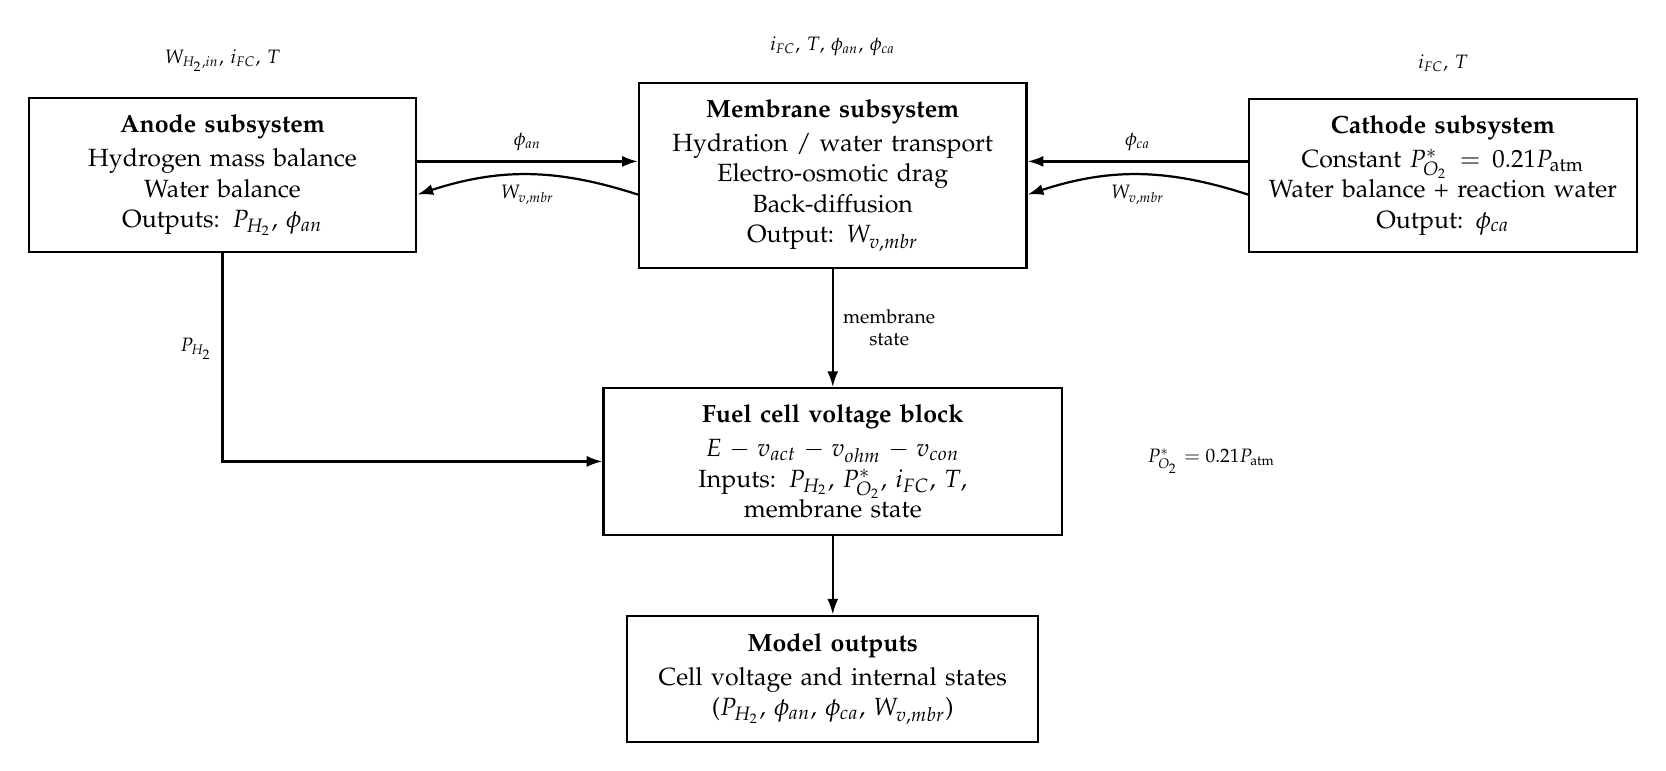
\begin{tikzpicture}[
    >=Latex,
    block/.style={draw, rectangle, thick, fill=white, align=center,
        text width=4.5cm, minimum height=1.9cm, inner sep=6pt, font=\small},
    vblock/.style={draw, rectangle, thick, fill=white, align=center,
        text width=5.4cm, minimum height=1.85cm, inner sep=6pt, font=\small},
    oblock/.style={draw, rectangle, thick, fill=white, align=center,
        text width=4.8cm, minimum height=1.6cm, inner sep=6pt, font=\small},
    lab/.style={font=\scriptsize, align=center},
    line/.style={-{Latex[length=2mm,width=1.4mm]}, line width=0.8pt}
]
\node[block] (anode) {\textbf{Anode subsystem}\\[0.15em]
Hydrogen mass balance\\ Water balance\\ Outputs: $P_{H_2},\,\phi_{an}$};
\node[block, right=2.8cm of anode] (membrane) {\textbf{Membrane subsystem}\\[0.15em]
Hydration / water transport\\ Electro-osmotic drag\\ Back-diffusion\\ Output: $W_{v,mbr}$};
\node[block, right=2.8cm of membrane] (cathode) {\textbf{Cathode subsystem}\\[0.15em]
Constant $P_{O_2}^{\ast}=0.21P_{\mathrm{atm}}$\\ Water balance + reaction water\\ Output: $\phi_{ca}$};
\node[vblock, below=1.50cm of membrane] (voltage) {\textbf{Fuel cell voltage block}\\[0.15em]
$E-v_{act}-v_{ohm}-v_{con}$\\ Inputs: $P_{H_2},\,P_{O_2}^{\ast},\,i_{FC},\,T,$ membrane state};
\node[oblock, below=1.0cm of voltage] (output) {\textbf{Model outputs}\\[0.15em]
Cell voltage and internal states\\ ($P_{H_2},\,\phi_{an},\,\phi_{ca},\,W_{v,mbr}$)};
\node[lab, above=0.2cm of anode] {$W_{H_2,in},\,i_{FC},\,T$};
\node[lab, above=0.2cm of membrane] {$i_{FC},\,T,\,\phi_{an},\,\phi_{ca}$};
\node[lab, above=0.2cm of cathode] {$i_{FC},\,T$};
\draw[line] ([yshift=5pt]anode.east) -- node[above,lab] {$\phi_{an}$} ([yshift=5pt]membrane.west);
\draw[line] ([yshift=-7pt]membrane.west) to[bend right=18]
    node[below,lab] {$W_{v,mbr}$} ([yshift=-7pt]anode.east);
\draw[line] ([yshift=5pt]cathode.west) -- node[above,lab] {$\phi_{ca}$} ([yshift=5pt]membrane.east);
\draw[line] ([yshift=-7pt]cathode.west) to[bend right=18]
    node[below,lab] {$W_{v,mbr}$} ([yshift=-7pt]membrane.east);
\draw[line] (anode.south) |- node[pos=0.23,left,lab] {$P_{H_2}$} (voltage.west);
\draw[line] (membrane.south) -- node[right,lab] {membrane\\state} (voltage.north);
\node[lab, right=0.95cm of voltage] {$P_{O_2}^{\ast}=0.21P_{\mathrm{atm}}$};
\draw[line] (voltage.south) -- (output.north);
\end{tikzpicture}%
}
\caption[Block-level architecture of the simplified PEMFC model]{Block-level
         architecture of the simplified PEMFC model. The anode, membrane, and
         cathode subsystems exchange water and feed the voltage block, which
         combines the Nernst potential with the three losses to produce the cell
         voltage. The diagram makes explicit which signals are inputs (top) and
         which are internal states.}
\label{fig:architecture}
\end{figure}

\subsection{Model Properties and Next Steps}
\label{sec:model-properties}

The preceding subsections define a compact model with a clear structure. Its
state vector is $\mathbf{x}=(P_{H_2},m_{w,an},m_{w,ca})$: the anode hydrogen
pressure and the water masses stored on each side of the membrane. Its inputs are
the load current $i_{FC}$, set by the external load and treated as a disturbance,
and the hydrogen inlet flow $W_{H_2,in}$, the manipulated input. Its single
measured output is the cell voltage of \eqref{eq:vfc}. Each cell carries six
calibration parameters, $\boldsymbol{\theta}=(\xi_1,\xi_2,\xi_3,\xi_4,B,c)$.

The model is deliberately simplified for control. The constant-$P_{O_2}$
assumption and the lumped volumes keep the order low, at the cost of ignoring
spatial gradients, oxygen transients, and liquid-water accumulation
\cite{weber2004,zhang2017}. This makes it well suited to fast simulation,
linearization, and controller design, while remaining accurate enough to match
each measured cell, as the results of Chapter~\ref{Chapter4} confirm.

These properties set the agenda for the rest of the methodology. First, the six
parameters are calibrated per cell (Section~\ref{sec:identification}). Next, the
model is linearized and its controllability and observability are analyzed
(Section~\ref{sec:ctrb-obsv}), which determines what can be controlled and
observed. The experimental protocols (Section~\ref{sec:protocols}) then provide
the dynamic data used to validate the model and to fix the timescales for the
control design of Chapter~\ref{Chapter5}.

\section{Per-Cell Parameter Identification}
\label{sec:identification}

The six parameters of each cell are identified by minimizing the root-mean-square
error (RMSE) between predicted and measured cell voltage over a calibration
window:
\begin{equation}
    \min_{\boldsymbol{\theta}}\;
    \sqrt{\frac{1}{N}\sum_{i=1}^{N}
        \bigl(v_{\text{model}}(I_i,P_{H_2,i};\boldsymbol{\theta})-v_{\text{meas},i}\bigr)^2}.
    \label{eq:rmse}
\end{equation}
Table~\ref{tab:opt-vars} lists the decision variables, their physical role, and
the box bounds used by the optimizer. The bounds also encode the physical
constraints $\xi_4\le 0$ (activation overvoltage grows with current),
$B\ge 0$, and $c\ge 0$ (losses are non-negative).

\begin{table}[t]
    \centering
    \caption[Optimization variables for the per-cell identification]{Decision
             variables of the per-cell identification problem \eqref{eq:rmse},
             with their role in the loss equations
             \eqref{eq:vact}--\eqref{eq:vcon} and the search bounds. The four
             $\xi$ coefficients shape the activation overvoltage; $B$ and $c$
             scale the concentration and contact-resistance losses.}
    \label{tab:opt-vars}
    \small
    \begin{tabular}{clcc}
        \toprule
        \textbf{Variable} & \textbf{Physical role} & \textbf{Unit} & \textbf{Search bounds} \\
        \midrule
        $\xi_1$ & Activation: constant term \eqref{eq:vact}            & V             & $[-8.0,\ 2.0]$ \\
        $\xi_2$ & Activation: temperature term                         & V\,K$^{-1}$   & $[0,\ 3\times10^{-2}]$ \\
        $\xi_3$ & Activation: oxygen-concentration term                & V\,K$^{-1}$   & $[-5\times10^{-3},\ 5\times10^{-3}]$ \\
        $\xi_4$ & Activation: current term ($\le 0$)                   & V\,K$^{-1}$   & $[-1\times10^{-2},\ 0]$ \\
        $B$     & Concentration-loss coefficient \eqref{eq:vcon}       & V             & $[0,\ 2.0]$ \\
        $c$     & Contact / lumped ohmic resistance \eqref{eq:vohm}    & $\Omega$      & $[0,\ 1\times10^{-2}]$ \\
        \bottomrule
    \end{tabular}
\end{table}

A two-stage strategy is used: \textbf{differential evolution} for the global
search (population~20, up to 800 generations, fixed seed), followed by
\textbf{L-BFGS-B} local refinement under the same bounds. Differential evolution
is a population-based global optimizer that needs no gradient, which suits the
non-convex objective; L-BFGS-B then polishes the best candidate. The optimizer
converges for most cells within a few tens of generations
(Figure~\ref{fig:cost-evolution}).

\begin{figure}[t]
    \centering
    
\includegraphics[width=0.95\linewidth]{Figures/cost_evolution_exp19.png}
    \caption[Differential-evolution convergence per cell]{Differential-evolution
             convergence (RMSE versus generation, log scale) for the ten cells.
             The dashed line marks the final RMSE after L-BFGS-B refinement. Most
             cells converge within a few tens of generations; the degraded cells
             (0--2) collapse almost immediately to a near-zero RMSE against a flat
             zero-voltage signal, which is the first sign of a degenerate fit.}
    \label{fig:cost-evolution}
\end{figure}

\section{State-Space Representation, Controllability and Observability}
\label{sec:ctrb-obsv}

To prepare for control and observer design, the model is linearized around an
operating point $(\mathbf{x}_0,\mathbf{u}_0)$ and written in the standard form
$\dot{\mathbf{x}}=A\mathbf{x}+B\mathbf{u}$, $y=C\mathbf{x}+D\mathbf{u}$.
Controllability is assessed through the rank of $\mathcal{C}=[B\;AB\;A^2B]$ and
observability through $\mathcal{O}=[C;\,CA;\,CA^2]$.

\subsection{State-Space Representation}

The linearized model uses the state, input, and output vectors
\begin{equation*}
    \mathbf{x} = \begin{bmatrix} P_{H_2} \\ m_{w,an} \\ m_{w,ca} \end{bmatrix},
    \qquad
    \mathbf{u} = \begin{bmatrix} i_{FC} \\ W_{H_2,in} \end{bmatrix},
    \qquad
    y = v_{fc},
\end{equation*}
where $P_{H_2}$ is the anode hydrogen partial pressure, $m_{w,an}$ and $m_{w,ca}$
the water masses stored on the anode and cathode sides, $i_{FC}$ the load current
(a disturbance imposed by the load), $W_{H_2,in}$ the hydrogen inlet flow (the
manipulated input), and $v_{fc}$ the measured cell voltage. The four matrices
have a direct physical reading: $A$ describes the internal dynamics (water
exchange across the membrane; the hydrogen pressure acts as an integrator), $B$
describes how the current drawn and the inlet flow drive the states, $C$
describes how the states appear in the measured voltage, and $D$ is the direct
feedthrough from the inputs to the voltage.

\subsubsection*{Matrices $A$ and $B$ --- read directly from the dynamic equations}
The three state equations of Section~\ref{sec:model} are linear in the states and
inputs once the temperature is held constant: the hydrogen pressure balance
\eqref{eq:anode} (with $W_{H_2,out}\approx 0$ for the dead-end anode) and the two
water balances written on the membrane water-transport terms,
\begin{equation*}
    \dot{m}_{w,an} = -\beta\, m_{w,an} + \gamma\, m_{w,ca} + d_1\, i_{FC},
    \qquad
    \dot{m}_{w,ca} = \beta\, m_{w,an} - \gamma\, m_{w,ca} + d_2\, i_{FC},
\end{equation*}
with
$\beta = D_w/(V_{an}t_m)$, $\gamma = D_w/(V_{ca}t_m)$,
$d_1 = n_d M_v/F$, and $d_2 = (n-2n_d)M_v/(2F)$.
No linearization is needed; the matrices follow immediately:
\begin{equation}
    A =
    \begin{bmatrix}
        0 & 0 & 0\\[2pt]
        0 & -\beta & \gamma\\[2pt]
        0 & \beta & -\gamma
    \end{bmatrix},
    \qquad
    B =
    \begin{bmatrix}
        -\dfrac{R_{H_2}T\,M_{H_2}\,n}{2F\,V_{an}} & \dfrac{R_{H_2}T}{V_{an}}\\[8pt]
        d_1 & 0\\[2pt]
        d_2 & 0
    \end{bmatrix}.
    \label{eq:AB}
\end{equation}
The first column of $B$ is the effect of the load current (hydrogen consumption
and electro-osmotic water displacement); the second column shows that the inlet
flow acts on the hydrogen pressure only.

\subsubsection*{Matrices $C$ and $D$ --- obtained by Jacobian linearization}
Unlike the state equations, the output equation
$y = v_{fc} = E(P_{H_2}) - v_{act}(i_{FC}) - v_{ohm}(i_{FC},\lambda_m(m_{w,an},m_{w,ca})) - v_{con}(i_{FC})$
is \emph{nonlinear} in both states and inputs --- it contains logarithms of
$P_{H_2}$ and $i_{FC}$ and the nonlinear membrane-resistivity law
\eqref{eq:vohm} --- so $C$ and $D$ cannot be read off the equations. They are
obtained by a first-order Taylor (Jacobian) expansion around the operating point
$(\mathbf{x}_0,\mathbf{u}_0)$:
\begin{equation*}
    \delta y \;\approx\;
    \underbrace{\left.\frac{\partial v_{fc}}{\partial \mathbf{x}}\right|_{(\mathbf{x}_0,\mathbf{u}_0)}}_{C}\,
    \delta\mathbf{x}
    \;+\;
    \underbrace{\left.\frac{\partial v_{fc}}{\partial \mathbf{u}}\right|_{(\mathbf{x}_0,\mathbf{u}_0)}}_{D}\,
    \delta\mathbf{u}.
\end{equation*}
The three steps are:
\begin{enumerate}[label=\arabic*)]
    \item \emph{Hydrogen-pressure entry.} Only the Nernst term \eqref{eq:ocv}
          depends on $P_{H_2}$:
          $\partial v_{fc}/\partial P_{H_2}
           = 4.31\times10^{-5}\,T/P_{H_2,0}$.
    \item \emph{Water-state entries.} The water masses act on the voltage through
          the chain
          $m_{w}\rightarrow \phi \rightarrow \lambda_m \rightarrow \sigma_m
           \rightarrow v_{ohm}$. Differentiating this chain gives
          \begin{equation*}
              \frac{\partial v_{fc}}{\partial m_{w,an}}
              = \kappa_0\,\lambda'(\phi_{an,0})\,\frac{R_v T}{2V_{an}p_{sat}(T)},
              \qquad
              \frac{\partial v_{fc}}{\partial m_{w,ca}}
              = \kappa_0\,\lambda'(\phi_{ca,0})\,\frac{R_v T}{2V_{ca}p_{sat}(T)},
          \end{equation*}
          with
          $\kappa_0 = i_0 t_m b_{11}
           \exp\bigl[b_2(\tfrac{1}{303}-\tfrac{1}{T})\bigr]/(A_{fc}\,\sigma_{m,0}^{2})$
          and $\lambda'(a)=17.81-79.70a+108a^2$ (derivative of the Springer
          isotherm).
    \item \emph{Input entries.} Differentiating the three loss terms with respect
          to $i_{FC}$ at $i_0$, and noting that $W_{H_2,in}$ does not enter the
          output equation directly:
          \begin{equation*}
              \frac{\partial v_{fc}}{\partial i_{FC}}
              = -\Bigl(\frac{\xi_4 T}{i_0}
                + \rho_{m,0}\frac{t_m}{A_{fc}} + c
                + \frac{B}{i_{\max}-i_0}\Bigr),
              \qquad
              \frac{\partial v_{fc}}{\partial W_{H_2,in}} = 0.
          \end{equation*}
\end{enumerate}
The resulting output matrices at the operating point are
\begin{equation}
    C =
    \begin{bmatrix}
        \dfrac{4.31\times10^{-5}\,T}{P_{H_2,0}} &
        \kappa_0\,\lambda'(\phi_{an,0})\,\dfrac{R_v T}{2V_{an}p_{sat}(T)} &
        \kappa_0\,\lambda'(\phi_{ca,0})\,\dfrac{R_v T}{2V_{ca}p_{sat}(T)}
    \end{bmatrix},
    \label{eq:Cmat}
\end{equation}
\begin{equation}
    D =
    \begin{bmatrix}
        -\Bigl(\dfrac{\xi_4 T}{i_0}
        + \rho_{m,0}\dfrac{t_m}{A_{fc}} + c
        + \dfrac{B}{i_{\max}-i_0}\Bigr) & 0
    \end{bmatrix}.
    \label{eq:Dmat}
\end{equation}
In the simplified model where $\lambda_m$ is held constant, the two water-state
entries of $C$ vanish and
$C_{\text{red}} = \bigl[\,4.31\times10^{-5}\,T/P_{H_2,0}\;\;0\;\;0\,\bigr]$.

\subsection{Controllability}

Because $P_{H_2}$ is directly driven by $W_{H_2,in}$ (entry
$R_{H_2}T/V_{an}>0$ in $B$), controllability of the full system reduces to
controllability of the two-state water subsystem
$(A_w,B_w)$ with
$A_w=\bigl[\begin{smallmatrix}-\beta & \gamma\\ \beta & -\gamma\end{smallmatrix}\bigr]$
and $B_w=[d_1;\,d_2]$ from \eqref{eq:AB}. Its controllability determinant,
$\det(\mathcal{C}_w)=(d_1+d_2)(\beta d_1-\gamma d_2)$ with
$d_1+d_2=nM_v/(2F)>0$, vanishes only under the single degenerate condition
\begin{equation}
    n_d = \frac{n\,V_{an}}{2\,(V_{an}+V_{ca})},
    \label{eq:ctrb-cond}
\end{equation}
i.e.\ when electro-osmotic drag exactly cancels the back-diffusion transport.
\textbf{The system is therefore fully controllable for all physically realistic
drag coefficients.}

\subsection{Observability}

With voltage as the only measurement, the observability matrix
$\mathcal{O}=[C;\,CA;\,CA^2]$ is built from \eqref{eq:Cmat}. In the simplified
model the output reduces to $C_{\text{red}}$, so the
\textbf{voltage observes the hydrogen pressure but not the two water states.}
In the full model all three states are potentially observable, but the
water-state sensitivities in \eqref{eq:Cmat} are small and degrade away from the
operating point. The practical consequence is that hydrogen-pressure regulation
can rely on a reduced-order voltage-based observer, whereas a full-state observer
would require additional pressure or humidity sensors.

\section{Experimental Protocols}
\label{sec:protocols}

All experiments were performed on the ten-cell educational PEMFC stack of the
laboratory bench, with per-cell voltage acquisition at 1\,Hz through the serial
data-acquisition chain developed in the project.
\begin{itemize}
    \item \textbf{Optimization Experiment} (April 2026): a fixed $25\,\Omega$
          resistor is connected at $t=135$\,s and removed at $t=684$\,s, with no
          valve-driven current control. The calibration points used for the
          per-cell parameter identification are drawn from the loaded window of
          this experiment.
    \item \textbf{TR-current step experiments} (9 June 2026): the stack is left at
          open circuit, then a fixed resistor ($3.3\,\Omega$ for Experiment~1,
          $6.8\,\Omega$ for Experiment~4) is connected at $t=0$. The processing
          pipeline detects the connection event from a $>100$\,mA current jump and
          re-zeros the time axis. The current step response is fitted with the
          exponential model
          $I(t)=I_{\text{ss}}+\Delta I\,e^{-t/\tau_I}$, from which settling times
          $T_{s,p\%}=-\tau_I\ln(p/100)$ are derived analytically; the
          90\,\%$\to$10\,\% fall time is measured on the raw signal.
\end{itemize}

% Chapter 4 — Results & Analysis

\chapter{Results \& Analysis}

\label{Chapter4}

\section{Parameter Identification on the Optimization Experiment}
\label{sec:results-identification}

The two-stage optimizer of Section~\ref{sec:identification} identified the six
parameters for all ten cells from the loaded window of the Optimization
Experiment. The complete set of tuned values is given in
Appendix~\ref{app:tables}, Table~\ref{tab:params-opt}. For the healthy cells the
calibration RMSE ranges from 2.0 to 11.3\,mV --- below 12\,mV in every case --- and
the mean time-series RMSE over the healthy cells is 8.0\,mV. These figures confirm
that a six-parameter law reproduces each cell to within a few millivolts.

Figure~\ref{fig:ts-opt-stack} places the experiment in context. The stack sits at
its open-circuit plateau of about 4.57\,V, drops to roughly 0.8\,V when the
$25\,\Omega$ resistor is connected at $t=135$\,s, draws a load current that decays
from about 30\,mA, and recovers when the resistor is removed at $t=684$\,s. The
simulated stack voltage (sum of the ten calibrated cells) tracks the measured
trace throughout the loaded window, which shows that the per-cell fits aggregate
correctly to the stack level.

\begin{figure}[t]
    \centering
    
\includegraphics[width=0.92\linewidth]{Figures/comparison_exp19_stack.png}
    \caption[Stack voltage and load current, Optimization Experiment]{Stack
             voltage and load current during the Optimization Experiment.
             \textbf{Top:} measured (blue) and simulated (red) stack voltage; the
             load is applied at $t=135$\,s and removed at $t=684$\,s.
             \textbf{Bottom:} the load current $I=V_{\text{stack}}/25\,\Omega$.
             The close overlap in the loaded window confirms that the calibrated
             cell models sum to the correct stack voltage.}
    \label{fig:ts-opt-stack}
\end{figure}

\begin{figure}[t]
    \centering
    
\includegraphics[width=\linewidth]{Figures/all_cells_overview_exp19.png}
    \caption[Per-cell voltage--current calibration fits]{Per-cell
             voltage--current calibration fits: measured points (blue) versus the
             identified model (red). The seven healthy cells (3--9) are matched
             with RMSE between 2.0 and 11.3\,mV. Cells~0--2 (highlighted) collapse
             to a near-zero voltage under load, so the optimizer cannot produce a
             meaningful curve --- a clear signature of hardware degradation.}
    \label{fig:vi-opt}
\end{figure}

The per-cell calibration fits in Figure~\ref{fig:vi-opt} explain these numbers.
Two findings stand out. First, the model describes the healthy cells accurately
with only six parameters: the activation coefficients are consistent across cells,
while the concentration ($B$) and contact-resistance ($c$) terms stay close to
zero, indicating that activation and ohmic effects dominate over the covered
range. Second, the identification doubles as a \emph{diagnosis} tool. Cells~0, 1,
and~2 collapse to about 0\,V under load, and the optimizer returns identical,
degenerate parameter sets for them (RMSE below 0.1\,mV against a flat near-zero
signal). This is the signature of a non-functioning electrode, not a physically
meaningful fit, because no parameter combination within the bounds can reproduce a
dead cell.

The time-series comparison in Figure~\ref{fig:ts-opt-cells} confirms the fit cell
by cell. The simulated voltage overlays the measurement for the healthy cells
across the loaded window, whereas Cells~0--2 remain pinned near zero. The slightly
larger residuals of Cells~7 and~9 stem from the load-on transient, which the
calibration window deliberately excludes; over the settled window the agreement is
within the reported RMSE.

\begin{figure}[t]
    \centering
    
\includegraphics[width=\linewidth]{Figures/comparison_exp19_cells.png}
    \caption[Per-cell voltage: measured vs.\ simulated]{Per-cell voltage,
             measured (blue) versus simulated (red), over the full experiment.
             Healthy cells (3--9) are tracked closely; the degraded cells~0--2
             stay near zero under load. Titles report the time-series RMSE over
             the loaded window (mean 8.0\,mV for the healthy cells).}
    \label{fig:ts-opt-cells}
\end{figure}

\section{Step-Response Characterization (TR-Current Experiments)}
\label{sec:results-tr}

The TR-current experiments characterize how fast the stack current settles after a
load step. In both runs, Cells~1 and~2 read about 0\,mV throughout the loaded
window, confirming the degradation first seen in the Optimization Experiment; the
other cells behave normally. Figure~\ref{fig:tr-experiments} shows the raw
channels for the two loads.

\begin{figure}[t]
    \centering
    \begin{subfigure}[t]{0.49\linewidth}
        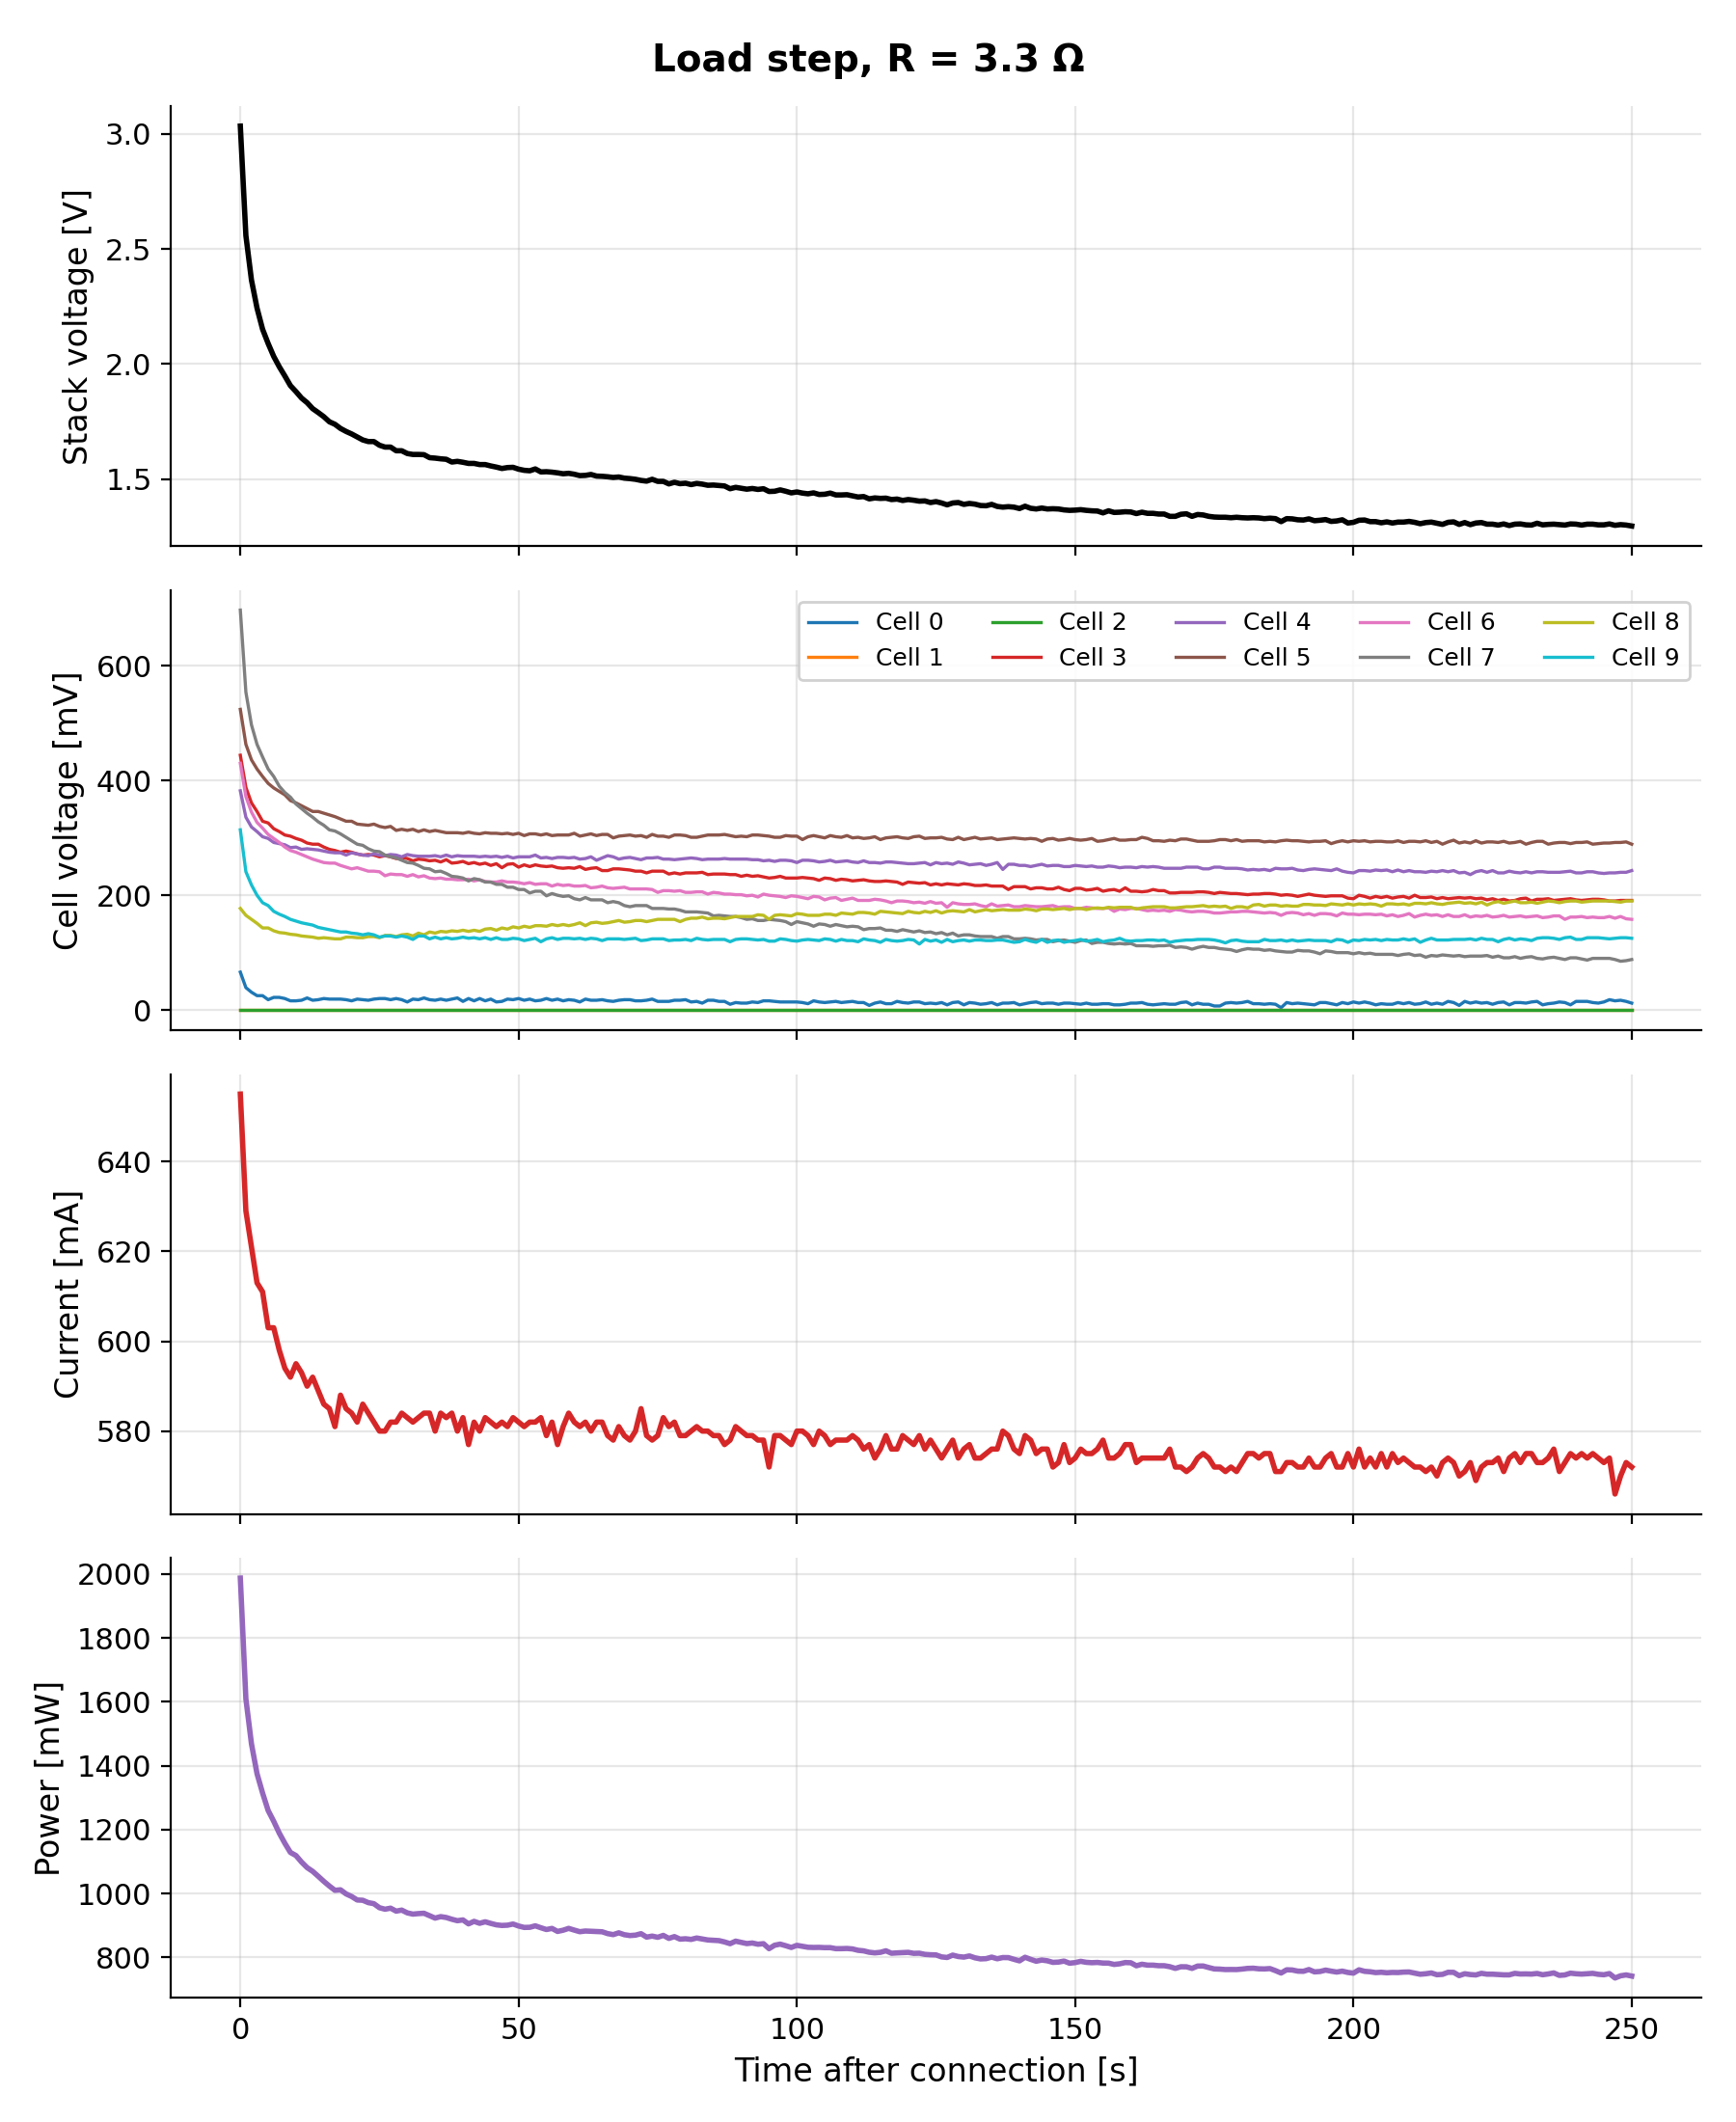
\includegraphics[width=\linewidth]{Figures/exp_33ohm_plot.png}
        \caption{Experiment~1, $R=3.3\,\Omega$.}
    \end{subfigure}\hfill
    \begin{subfigure}[t]{0.49\linewidth}
        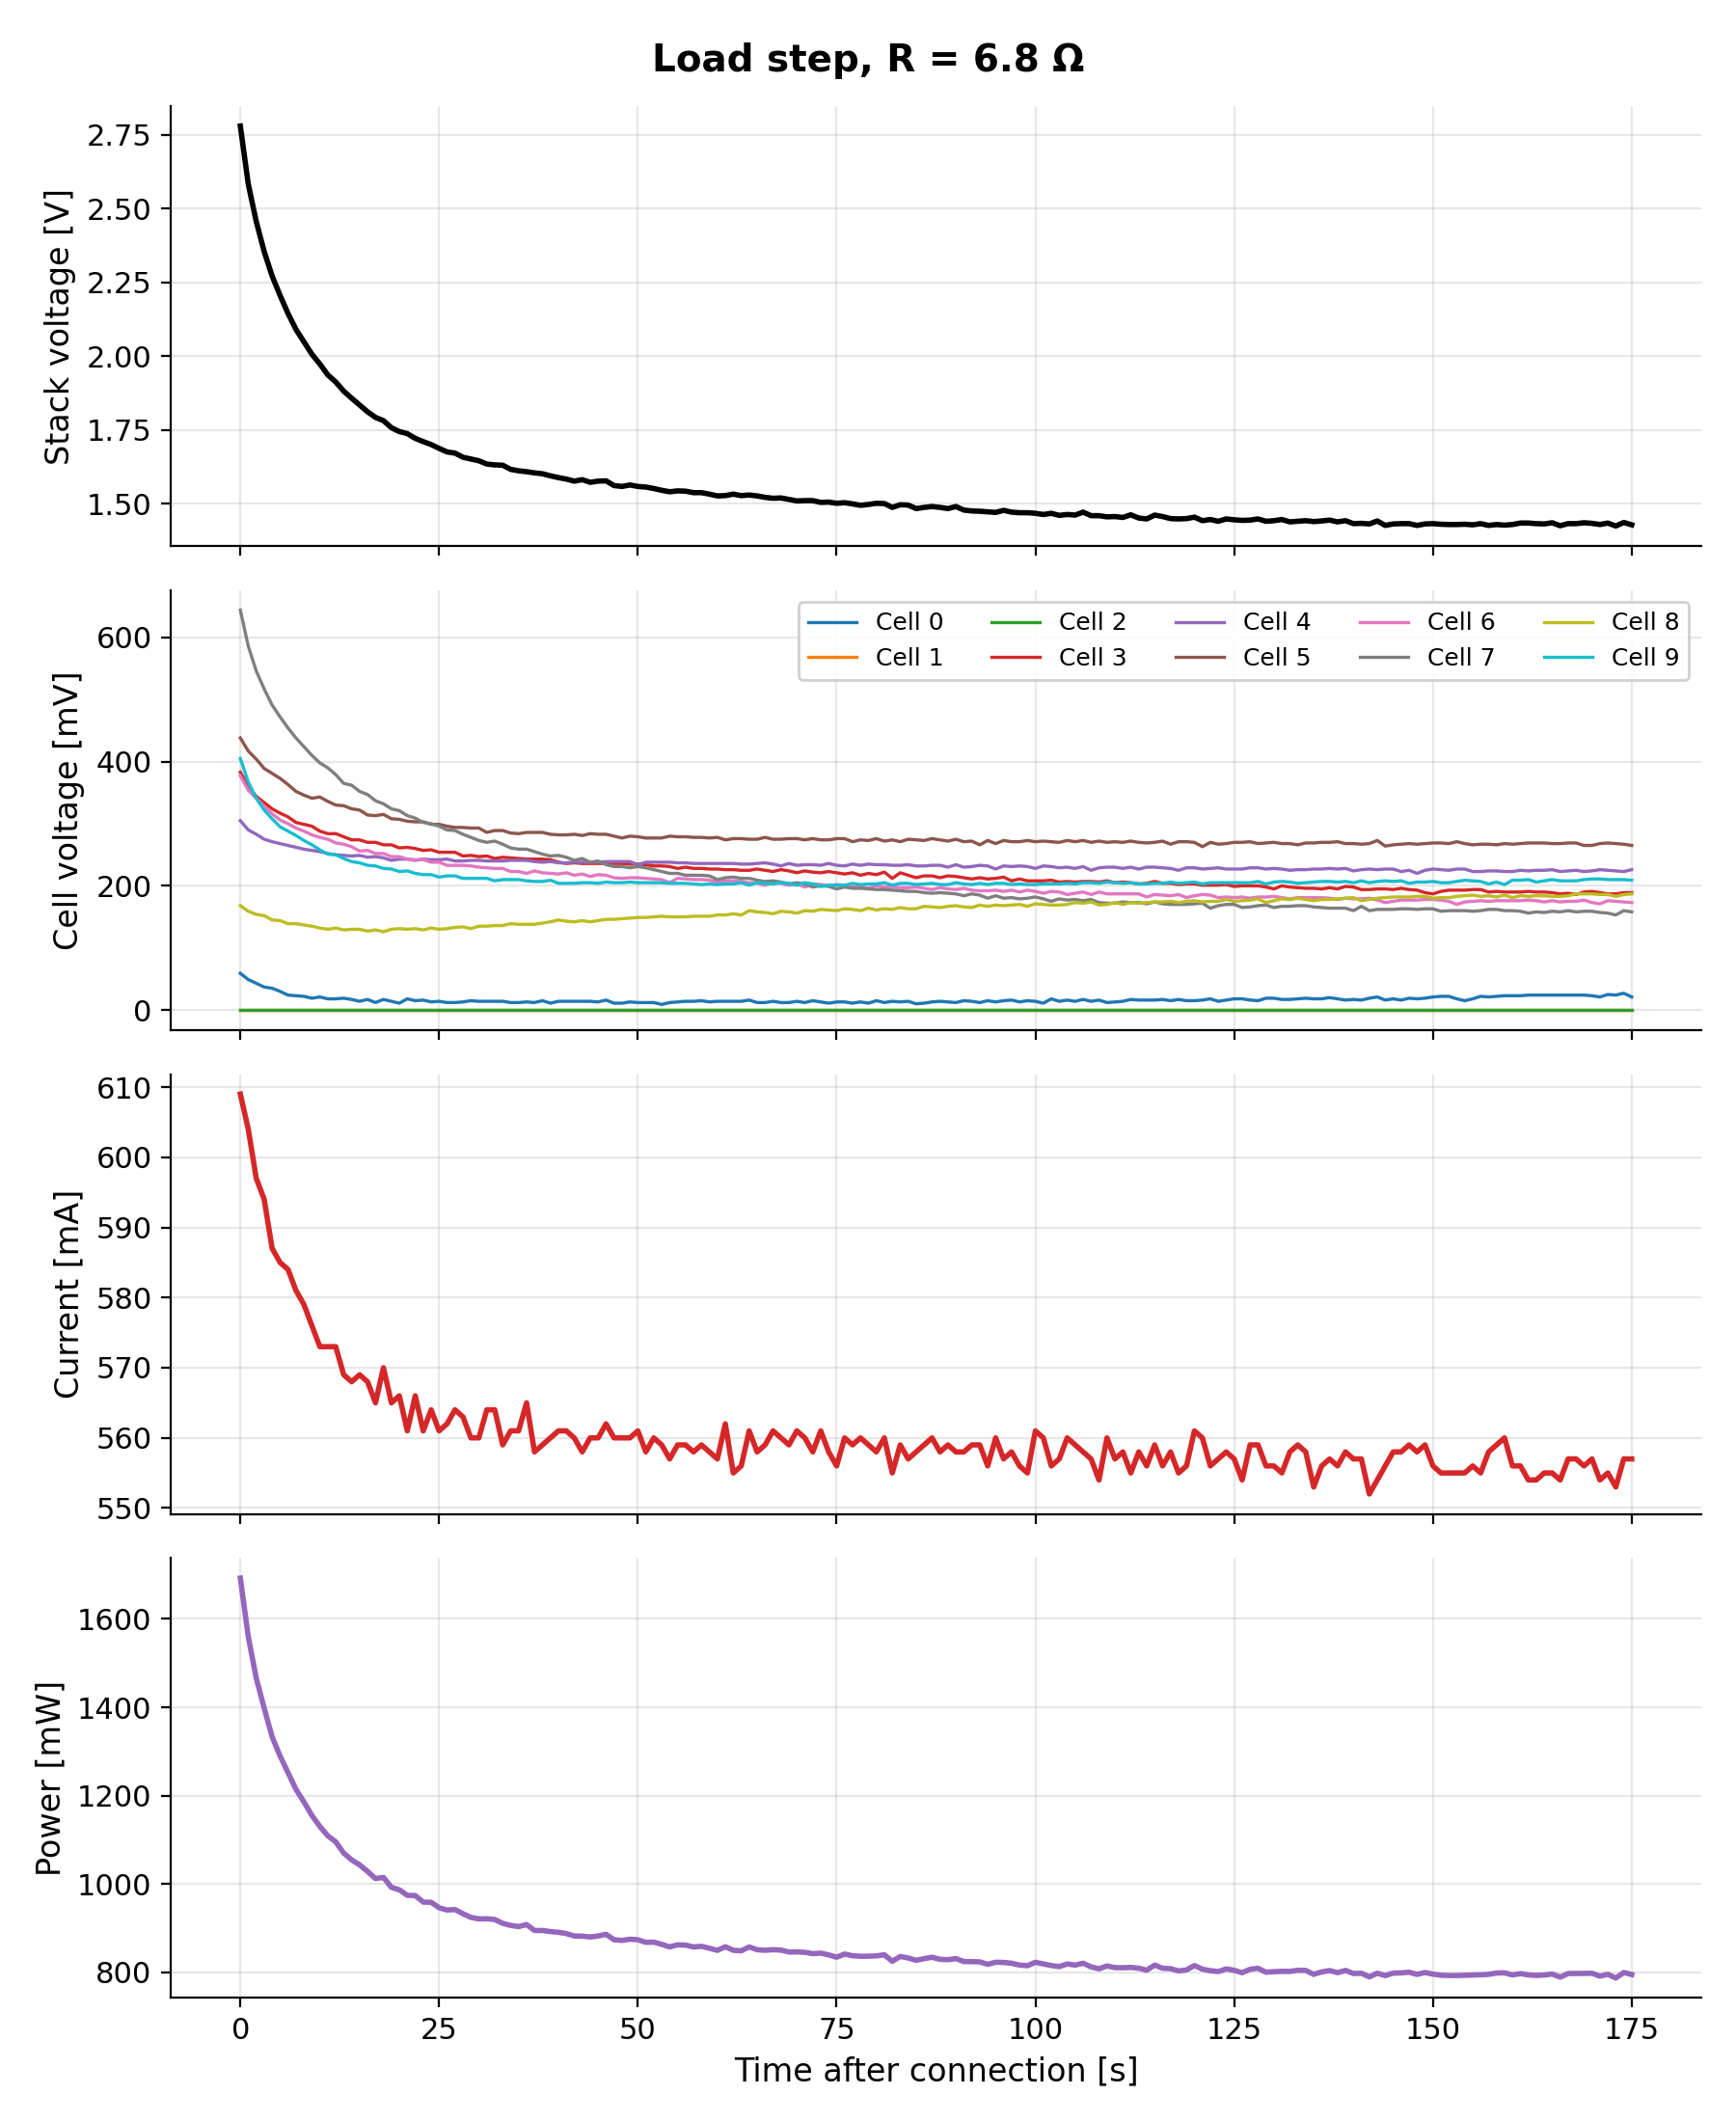
\includegraphics[width=\linewidth]{Figures/exp_68ohm_plot.png}
        \caption{Experiment~4, $R=6.8\,\Omega$.}
    \end{subfigure}
    \caption[TR-current step experiments]{TR-current step experiments after
             resistor connection (time re-zeroed to the step): stack voltage,
             individual cell voltages, current, and power. Both signals relax
             monotonically toward a steady state, with no overshoot --- behavior
             well captured by a first-order model.}
    \label{fig:tr-experiments}
\end{figure}

Fitting the first-order model $I(t)=I_{\text{ss}}+\Delta I\,e^{-t/\tau_I}$ to the
current gives the metrics of Table~\ref{tab:response-rt}, illustrated in
Figure~\ref{fig:tr-responses}.

\begin{table}[H]
    \centering
    \caption[Current step-response metrics]{Current step-response metrics for the
             two loads. The lighter load ($6.8\,\Omega$) gives a longer time
             constant and a smaller initial perturbation, consistent with slower
             dynamics at lower current density.}
    \label{tab:response-rt}
    \small
    \begin{tabular}{lcc}
        \toprule
        \textbf{Current metric} & \textbf{Exp~1 (3.3\,$\Omega$)} & \textbf{Exp~4 (6.8\,$\Omega$)} \\
        \midrule
        Steady-state current $I_{\text{ss}}$ [mA] & 572.9 & 556.1 \\
        Step amplitude $\Delta I$ [mA]             &  82.1 &  52.9 \\
        Time constant $\tau_I$ [s]                 &   8.2 &  10.3 \\
        Settling time $T_{s,2\%}$ [s]              &  32.0 &  40.2 \\
        Fall time 90\%$\to$10\% [s]                &  16.0 &  19.0 \\
        \bottomrule
    \end{tabular}
\end{table}

\begin{figure}[t]
    \centering
    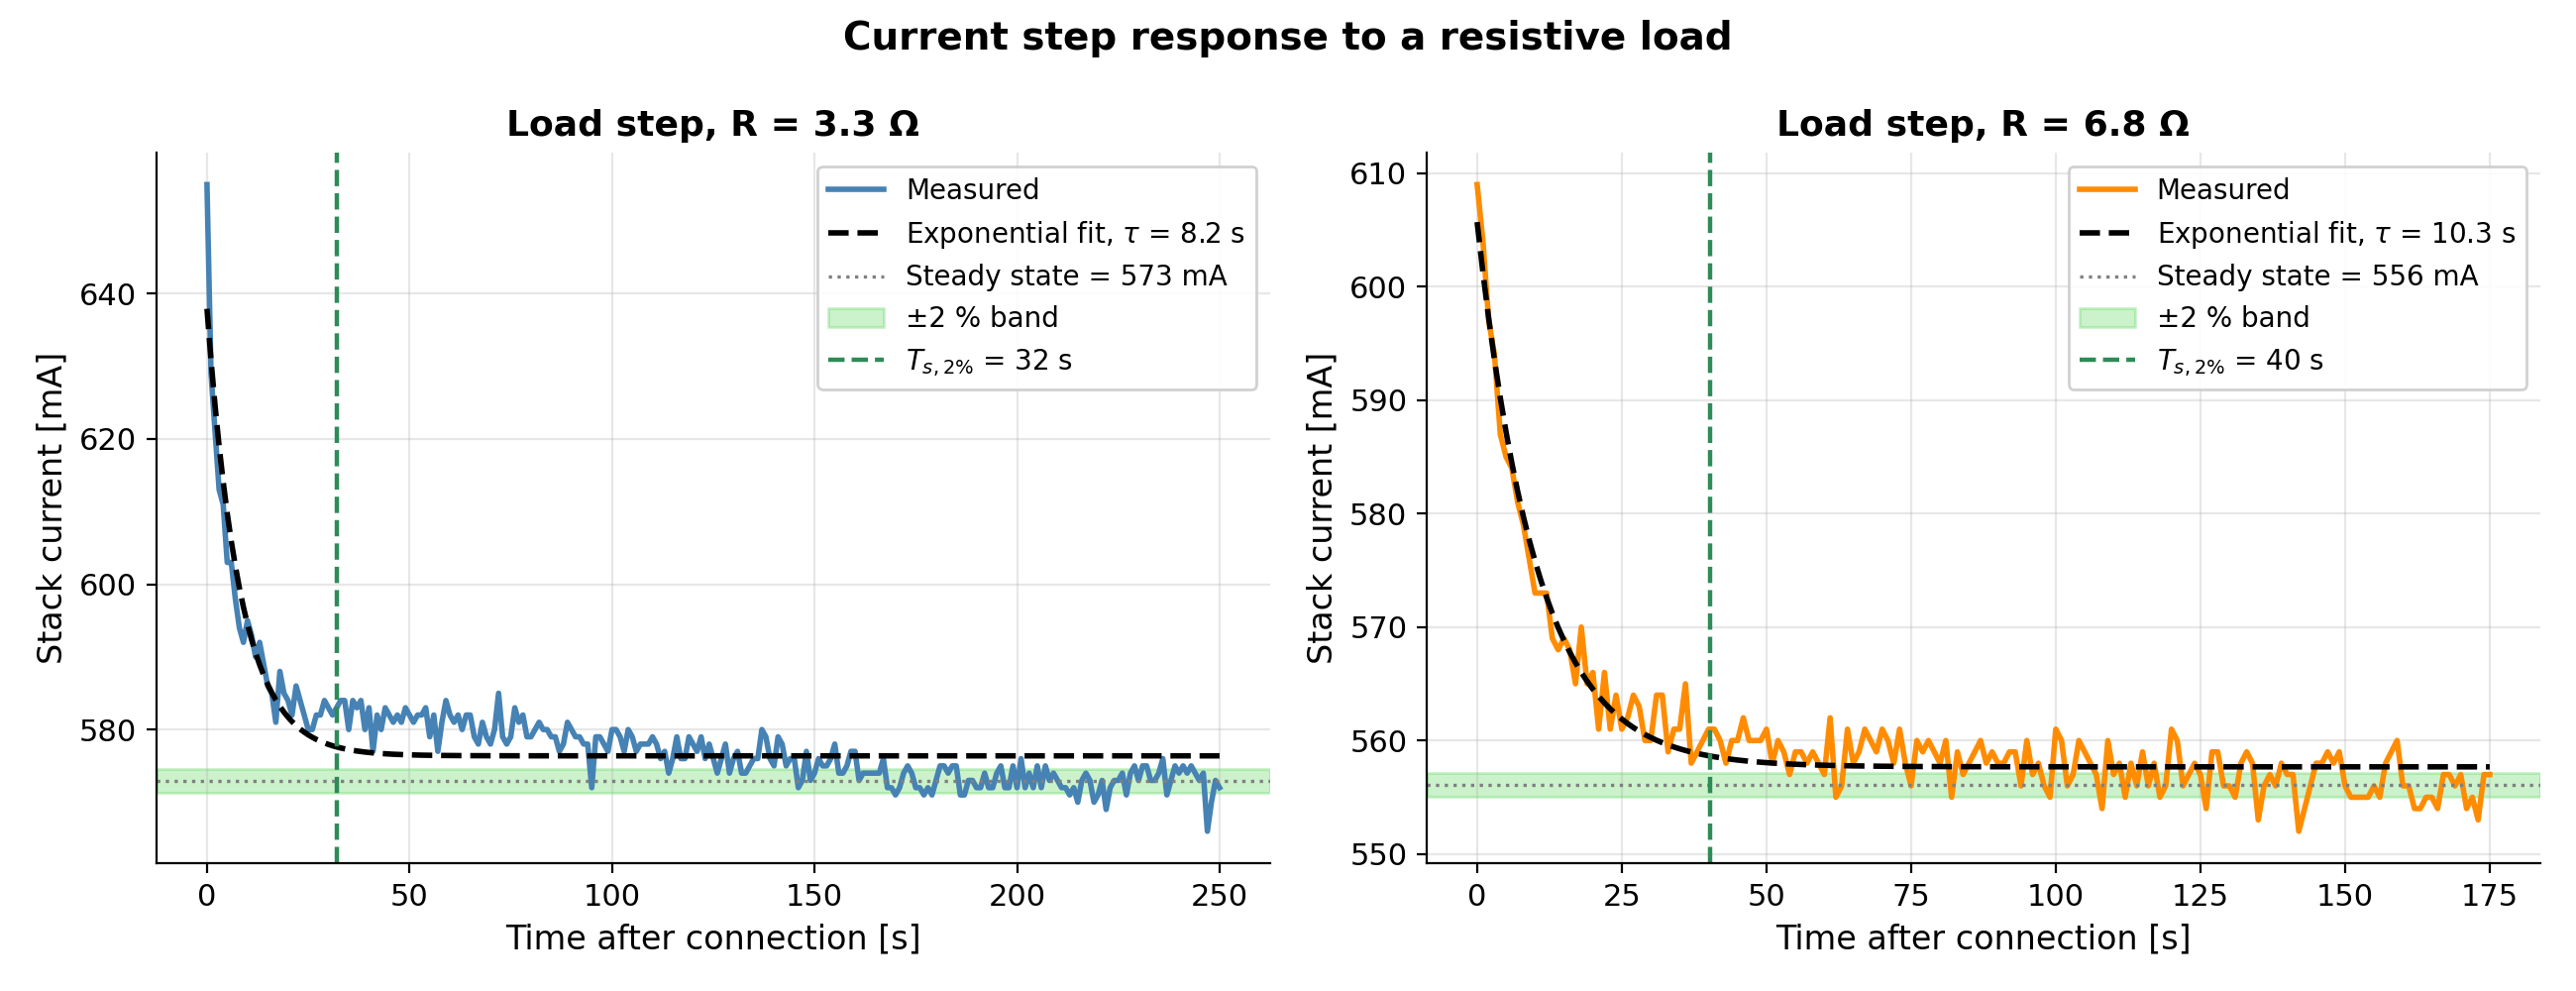
\includegraphics[width=0.95\linewidth]{Figures/response_time_plot.png}
    \caption[Current step response and exponential fit]{Current step response for
             the two loads: measured current (color), exponential fit (dashed),
             steady-state level, $\pm2\,\%$ settling band, and the 2\,\% settling
             time. The exponential model matches the data closely, justifying the
             first-order time constants reported in Table~\ref{tab:response-rt}.}
    \label{fig:tr-responses}
\end{figure}

The current time constant is about 25\,\% longer under the lighter load
($\tau_I=10.3$\,s at $6.8\,\Omega$ versus $8.2$\,s at $3.3\,\Omega$), consistent
with slower electrochemical dynamics at lower current density; the initial
perturbation $\Delta I$ is also smaller (52.9 versus 82.1\,mA). The settling times
derived from the fit ($T_{s,2\%}=32$--$40$\,s) are robust to measurement noise,
because they are computed analytically from $\tau_I$ rather than read off the
noisy raw signal. This timescale captures the dominant dynamics seen by the load
--- electrochemical kinetics combined with gas-supply transients --- and sets a
quantitative target for controller bandwidth: the closed-loop controller of
Chapter~\ref{Chapter5} must act well within $\tau_I\approx 8$--$10$\,s to shape the
stack's transient behavior.

% Chapter 5 — Control of the PEMFC Power System

\chapter{Control of the PEMFC Power System: DC/DC Boost Converter with PI Controller}

\label{Chapter5}

This chapter presents the control architecture adopted for the PEMFC power
system. As motivated in Section~\ref{sec:challenges}, the hydrogen supply offers
too little authority to regulate the load directly, so control is applied on the
electrical side through a DC/DC converter. The design follows the approach of
Derbeli et al.\ \cite{derbeli2017}.

\section{System Overview}
\label{sec:control-overview}

By itself, a PEMFC stack is \emph{neither} an ideal voltage source \emph{nor} an
ideal current source: its terminal voltage $V_{STACK}$ is low and varies strongly
with the current drawn, following the polarization curve of
Chapter~\ref{Chapter2}. The role of the control stage is to shape this raw output
into a \emph{regulated source}. The stack feeds a \textbf{DC/DC boost converter}
(a step-up chopper), and a \textbf{PI controller} closes the loop by acting on the
converter duty cycle $T$ through pulse-width modulation (PWM)
\cite{derbeli2017}. Figure~\ref{fig:boost-architecture} shows the architecture.

Depending on which variable the PI loop regulates, the \emph{converter output}
--- i.e.\ the PEMFC power system seen from the load --- can be made to behave as:
\begin{itemize}
    \item a \textbf{controlled current source} --- the loop regulates the
          inductor (stack) current $I_L$ to a reference $I_{REF}$
          (Section~\ref{sec:control-current});
    \item a \textbf{controlled voltage source} --- the loop regulates the output
          voltage $V_{OUT}$ to a reference $V_{REF}$
          (Section~\ref{sec:control-voltage}).
\end{itemize}
It is therefore the regulated converter output, not the fuel cell itself, that is
made to act as a current or a voltage source.

\begin{figure}[t]
\centering
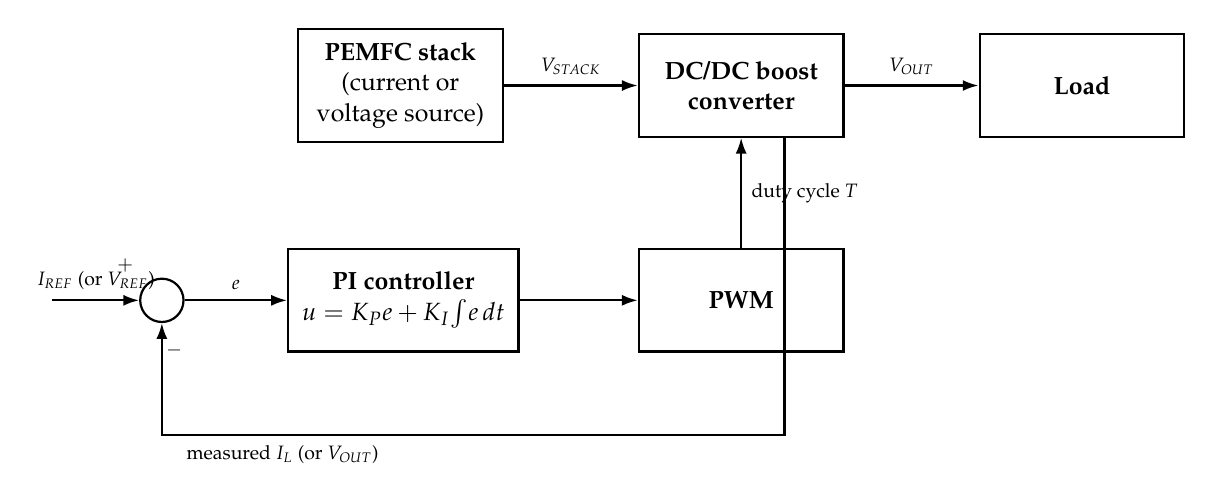
\begin{tikzpicture}[
    >=Latex,
    blk/.style={draw, rectangle, thick, fill=white, align=center,
        minimum height=1.3cm, minimum width=2.6cm, inner sep=5pt, font=\small},
    sums/.style={draw, circle, thick, minimum size=0.55cm, inner sep=0pt},
    lab/.style={font=\scriptsize, align=center},
    line/.style={-{Latex[length=2mm,width=1.4mm]}, line width=0.8pt}
]
\node[blk] (fc) {\textbf{PEMFC stack}\\ (current or\\ voltage source)};
\node[blk, right=1.7cm of fc] (boost) {\textbf{DC/DC boost}\\ \textbf{converter}};
\node[blk, right=1.7cm of boost] (load) {\textbf{Load}};
\node[blk, below=1.4cm of boost] (pwm) {\textbf{PWM}};
\node[blk, left=1.5cm of pwm] (pi) {\textbf{PI controller}\\ $u=K_P e + K_I\!\int\! e\,dt$};
\node[sums, left=1.3cm of pi] (sumj) {};
\node[lab, above left=1pt and 1pt of sumj.north west] {$+$};
\node[lab, below right=4pt and -2pt of sumj.south] {$-$};

\draw[line] (fc) -- node[above,lab] {$V_{STACK}$} (boost);
\draw[line] (boost) -- node[above,lab] {$V_{OUT}$} (load);
\draw[line] (pwm) -- node[right,lab] {duty cycle $T$} (boost);
\draw[line] (pi) -- (pwm);
\draw[line] (sumj) -- node[above,lab] {$e$} (pi);
\draw[line] ([xshift=-1.1cm]sumj.west) -- node[above,lab] {$I_{REF}$ (or $V_{REF}$)} (sumj);
\draw[line] ([xshift=0.55cm]boost.south) |- ([yshift=-1.05cm]pi.south)
    -| node[pos=0.25,below,lab] {measured $I_L$ (or $V_{OUT}$)} (sumj);
\end{tikzpicture}
\caption[Control architecture of the PEMFC power system]{Control architecture of
         the PEMFC power system, after \cite{derbeli2017}: the stack feeds a DC/DC
         boost converter whose duty cycle is set by a PI controller. Regulating
         the inductor current $I_L$ makes the converter output behave as a current
         source; regulating the output voltage $V_{OUT}$ makes it behave as a
         voltage source.}
\label{fig:boost-architecture}
\end{figure}

\section{Output Current Regulation (Current-Source Operation)}
\label{sec:control-current}

Here the goal is to make the regulated converter output behave as a
\textbf{current source}. Following \cite{derbeli2017}, the design proceeds in five
steps.

\begin{enumerate}[label=\arabic*)]
    \item \emph{Control objective.} The controlled variable is the inductor
          (stack) current $I_L$, which the PI loop forces to track a reference
          $I_{REF}$ so that the system delivers a regulated current. In the
          reference design, $I_{REF}=9.74$\,A is the maximum-power operating point
          of the 50\,W, ten-cell stack used for validation (54\,W at 5.54\,V).
          Regulating the current directly also protects the stack, whose maximum
          current (10\,A) must never be exceeded.
    \item \emph{Boost converter state-space model.} Averaging the two switching
          topologies of the converter (switch ON / switch OFF) over one PWM
          period yields, with state $x=[\,i_L \;\; V_{OUT}\,]^{\top}$, duty
          cycle $T$, load $R$, inductance $L$, and capacitance $C$
          \cite{derbeli2017}:
          \begin{equation}
              \dot{x} =
              \begin{bmatrix}
                  0 & \dfrac{T-1}{L} \\[8pt]
                  \dfrac{1-T}{C} & -\dfrac{1}{RC}
              \end{bmatrix} x
              +
              \begin{bmatrix}
                  \dfrac{1}{L} \\[6pt] 0
              \end{bmatrix} u,
              \qquad
              y = \begin{bmatrix} 0 & 1 \end{bmatrix} x.
              \label{eq:boost-ss}
          \end{equation}
    \item \emph{PI control law.} The error signal is $e = I_{REF} - I_L$, and
          the control output (duty cycle) combines proportional and integral
          action:
          \begin{equation}
              u = K_P\, e + K_I \!\int\! e \, dt.
              \label{eq:pi-law}
          \end{equation}
          The proportional term shapes the rise time and the integral term
          removes the steady-state error, at the cost of possible overshoot if the
          gains are too aggressive.
    \item \emph{PI tuning (online method).} The gains are tuned experimentally,
          without knowledge of the plant transfer function \cite{derbeli2017}:
          set $K_P=0$ and $T_i=\infty$; increase $K_P$ until sustained
          oscillations appear and note this value $K_{PU}$; set
          $K_P = K_{PU}/2$; then decrease $T_i$ until oscillations reappear
          ($T_{iU}$) and set $T_i = 2\,T_{iU}$.
    \item \emph{Expected behavior.} With properly tuned gains, the PI controller
          produces a smooth, stable rise of $I_L$ to $I_{REF}$ ($\approx 400$\,ms
          in the reference design) and good disturbance rejection under large load
          variations, as validated on a dSPACE~1104 real-time platform
          \cite{derbeli2017}.
\end{enumerate}

\section{Output Voltage Regulation (Voltage-Source Operation)}
\label{sec:control-voltage}

Here the goal is to make the same regulated converter output behave instead as a
\textbf{voltage source}, using the same PI-based methodology.

\begin{enumerate}[label=\arabic*)]
    \item \emph{Control objective.} The controlled variable is now the converter
          output voltage $V_{OUT}$, which the PI loop forces to track a reference
          $V_{REF}$ so that the system delivers a regulated voltage to the load.
    \item \emph{Boost converter model.} The same averaged state-space model
          \eqref{eq:boost-ss} applies; the output of interest is the second
          state, $y = V_{OUT}$.
    \item \emph{PI control law.} The error signal becomes
          $e = V_{REF} - V_{OUT}$, and the same control law \eqref{eq:pi-law}
          applies.
    \item \emph{Tuning.} The same online procedure is used, adapted to the
          voltage-loop dynamics, which include the $RC$ output stage and are
          therefore slower than the current loop.
    \item \emph{Comparison of the two objectives.} Regulating the current is
          better suited to protecting the PEMFC from overcurrent, since the
          controlled variable is the current drawn from the stack; regulating the
          output voltage is more natural for supplying a fixed voltage to the
          load. Both make the converter output behave as a regulated source, rely
          on the same PI structure and converter model, and differ only in the
          feedback variable ($I_L$ vs.\ $V_{OUT}$) and in the physical meaning of
          the reference.
\end{enumerate}

% Chapter 6 — Conclusion & Perspectives

\chapter{Conclusion \& Perspectives}

\label{Chapter6}

This work developed a simplified control-oriented model of a ten-cell PEMFC stack,
calibrated it per cell on the Optimization Experiment, derived and analyzed its
linearized state-space representation, characterized its dynamic current response
to load steps, and proposed a PI-based control architecture for the PEMFC power
system.

The main outcomes are: (i)~a six-parameter semi-empirical voltage model coupled to
lumped anode, membrane, and cathode dynamics that fits all healthy cells to within
12\,mV; (ii)~a diagnosis capability --- degraded cells (0, 1, 2) are revealed both
by voltage collapse and by degenerate, physically meaningless fits;
(iii)~an explicit state-space representation in which $A$ and $B$ follow directly
from the dynamic equations while $C$ and $D$ require Jacobian linearization of the
nonlinear voltage equation, leading to proof that the model is generically
controllable while a voltage-only observer can reconstruct the hydrogen pressure
but not the water states; (iv)~an experimental characterization of the current
response to load steps ($\tau_I\approx 8$--$10$\,s,
$T_{s,2\%}\approx 32$--$40$\,s); and (v)~a control architecture based on a DC/DC
boost converter regulated by a PI controller \cite{derbeli2017}, motivated by the
limited authority of the hydrogen supply, in which the converter output is
regulated to behave either as a current source (overcurrent protection) or as a
voltage source (output-voltage regulation).

Perspectives follow directly. On the control side, the next step is to implement
the proposed boost-converter PI loop on the bench and tune it online following
\cite{derbeli2017}, with the identified current timescale bounding the required
closed-loop bandwidth; the observability analysis further supports a
hydrogen-pressure regulator with a reduced-order voltage-based observer, with PI
control as the literature-standard baseline \cite{zhu2017,derbeli2017} and LQ or
time-delay control as upgrades \cite{pukrushpan2003,kim2010}. On the modeling
side, capturing oxygen transients (removing the constant-$P_{O_2}$ assumption),
liquid-water accumulation, and gas-supply delays \cite{kharrat2025} would extend
validity at higher dynamics. Finally, replacing the degraded cells and repeating
the calibration would allow stack-level closed-loop experiments.


%----------------------------------------------------------------------------------------
%	BIBLIOGRAPHY
%----------------------------------------------------------------------------------------
\bibliographystyle{plain}
\bibliography{example}

%----------------------------------------------------------------------------------------
%	THESIS CONTENT - APPENDICES
%----------------------------------------------------------------------------------------

\appendix % Cue to tell LaTeX that the following "chapters" are Appendices

% Include the appendices of the thesis as separate files from the Appendices folder

% Appendix A — OCV Thermodynamic Derivation

\chapter{Derivation of the Open-Circuit Voltage}

\label{app:ocv}

The global hydrogen--oxygen reaction is
$\mathrm{H_2+\tfrac{1}{2}O_2\rightarrow H_2O}$. At non-standard conditions the
Gibbs free energy change is
\[
    \Delta g_f = \Delta g_f^0
    - \bar{R}T_{fc}\ln\!\left(\frac{p_{H_2}\,p_{O_2}^{1/2}}{p_{H_2O}}\right),
\]
and for a reversible cell $\Delta g_f=-2FE$, so
\[
    E = -\frac{\Delta g_f^0}{2F}
      + \frac{\bar{R}T_{fc}}{2F}
        \ln\!\left(\frac{p_{H_2}\,p_{O_2}^{1/2}}{p_{H_2O}}\right).
\]

\section*{Standard Voltage}

Taking liquid water as the product at $25\,^{\circ}$C:
\[
    E^0=-\frac{\Delta g_f^0}{2F}
       =-\frac{-237{,}200}{2\times 96{,}485}\approx 1.229\;\mathrm{V}.
\]
Table~\ref{tab:gibbs} lists $\Delta g_f^0$ at several temperatures.

\begin{table}[H]
\centering
\caption{Gibbs free energy change of the hydrogen fuel cell reaction at various temperatures \cite{pukrushpan2003}.}
\label{tab:gibbs}
\begin{tabular}{ccc}
\toprule
\textbf{Product} & \textbf{Temperature ($^{\circ}$C)} & $\boldsymbol{\Delta g_f^0}$ \textbf{(kJ/mol)} \\
\midrule
Liquid & 25   & $-237.2$ \\
Liquid & 80   & $-228.2$ \\
Gas    & 80   & $-226.1$ \\
Gas    & 100  & $-225.2$ \\
Gas    & 200  & $-220.4$ \\
Gas    & 600  & $-199.6$ \\
Gas    & 1000 & $-177.4$ \\
\bottomrule
\end{tabular}
\end{table}

\section*{Temperature Coefficient}

From $\Delta G^0=\Delta H^0-T\Delta S^0$, with
\[
    \Delta S^0 = S^0_{\mathrm{H_2O(l)}} - S^0_{\mathrm{H_2(g)}}
               - \tfrac{1}{2}S^0_{\mathrm{O_2(g)}}
              = 69.95-130.7-102.58 \approx -163.3\;\mathrm{J\,mol^{-1}K^{-1}}
\]
for the liquid-water reaction,
\[
    \frac{\Delta S^0}{2F}\approx\frac{-163.3}{192{,}970}
    \approx -0.85\times10^{-3}\;\mathrm{V\,K^{-1}}.
\]

\section*{Nernst Pressure Correction}

Assuming $p_{H_2O}=1$ (liquid product):
\[
    \frac{\bar{R}T_{fc}}{2F}\ln\!\bigl(p_{H_2}\,p_{O_2}^{1/2}\bigr)
    = \frac{8.314\,T_{fc}}{192{,}970}
      \left[\ln p_{H_2}+\tfrac{1}{2}\ln p_{O_2}\right]
    \approx 4.31\times10^{-5}\,T_{fc}
      \left[\ln p_{H_2}+\tfrac{1}{2}\ln p_{O_2}\right].
\]

\section*{Final Expression}

Combining all terms yields Equation~\eqref{eq:ocv} of the main text:
\[
    E = 1.229 - 0.85\times10^{-3}(T_{fc}-298.15)
          + 4.31\times10^{-5}\,T_{fc}\!\left[\ln p_{H_2}+\tfrac{1}{2}\ln p_{O_2}\right]\;\text{V}.
\]

% Appendix C — Detailed Tables

\chapter{Detailed Tables}

\label{app:tables}

\begin{table}[H]
    \centering
    \caption{Tuned parameters and calibration RMSE for all ten cells ---
             Optimization Experiment. Cells~0--2 collapsed under load: the
             optimizer returns identical degenerate parameter sets that
             reproduce a near-zero voltage and are not physically meaningful.}
    \label{tab:params-opt}
    \small
    \begin{tabular}{lrrrrrrr}
        \toprule
        Cell & RMSE [mV] & $\xi_1$ & $\xi_2$ & $\xi_3$ & $\xi_4$ & $B$ & $c$ \\
        \midrule
        Cell~0$^{\dagger}$ & 0.08 & $-7.783$ & $1.67\!\times\!10^{-2}$ & $-6.06\!\times\!10^{-4}$ & $\approx 0$ & $1.08\!\times\!10^{-2}$ & $1.00\!\times\!10^{-2}$ \\
        Cell~1$^{\dagger}$ & 0.08 & $-7.783$ & $1.67\!\times\!10^{-2}$ & $-6.06\!\times\!10^{-4}$ & $\approx 0$ & $1.08\!\times\!10^{-2}$ & $1.00\!\times\!10^{-2}$ \\
        Cell~2$^{\dagger}$ & 0.08 & $-7.783$ & $1.67\!\times\!10^{-2}$ & $-6.06\!\times\!10^{-4}$ & $\approx 0$ & $1.08\!\times\!10^{-2}$ & $1.00\!\times\!10^{-2}$ \\
        Cell~3 &  4.66 & $-1.977$ & $2.83\!\times\!10^{-2}$ & $1.32\!\times\!10^{-3}$  & $-3.17\!\times\!10^{-4}$ & $\approx 0$ & $\approx 0$ \\
        Cell~4 &  2.18 & $ 0.386$ & $1.43\!\times\!10^{-2}$ & $8.11\!\times\!10^{-4}$  & $-1.24\!\times\!10^{-4}$ & $\approx 0$ & $\approx 0$ \\
        Cell~5 &  4.23 & $ 0.682$ & $3.00\!\times\!10^{-2}$ & $1.93\!\times\!10^{-3}$  & $-2.98\!\times\!10^{-4}$ & $\approx 0$ & $\approx 0$ \\
        Cell~6 &  4.51 & $ 1.775$ & $4.62\!\times\!10^{-3}$ & $4.87\!\times\!10^{-4}$  & $-2.73\!\times\!10^{-4}$ & $\approx 0$ & $\approx 0$ \\
        Cell~7 &  5.62 & $ 1.796$ & $2.54\!\times\!10^{-2}$ & $1.82\!\times\!10^{-3}$  & $-1.99\!\times\!10^{-4}$ & $\approx 0$ & $\approx 0$ \\
        Cell~8 &  1.96 & $-4.946$ & $2.81\!\times\!10^{-2}$ & $6.92\!\times\!10^{-4}$  & $-1.34\!\times\!10^{-4}$ & $\approx 0$ & $\approx 0$ \\
        Cell~9 & 11.25 & $-5.400$ & $2.01\!\times\!10^{-2}$ & $9.31\!\times\!10^{-5}$  & $-1.06\!\times\!10^{-4}$ & $3.21\!\times\!10^{-7}$ & $\approx 0$ \\
        \bottomrule
    \end{tabular}

    \medskip
    \footnotesize $^{\dagger}$ Degraded cell (voltage collapse under load); fit not physically meaningful.
\end{table}

% Appendix — Source Code

\chapter{Source Code}

\label{app:source}

The complete source code developed during this internship is available on GitHub.
It gathers the simplified PEMFC model, the per-cell parameter-identification
scripts (differential evolution + L-BFGS-B), the experiment-processing and
figure-generation pipelines, and the \LaTeX{} sources of this report and of the
defense presentation:

\begin{center}
    \large
    \url{https://github.com/KhalilEllahLAGHA/PEMFC_Internship_codes}
\end{center}


%----------------------------------------------------------------------------------------

\end{document}
